\section{Retail Gasoline: Dynamic Pricing, Price Cycles and a Prosecuted Cartel}\label{sec:13-gasoline}

Each case so far had a dated institution to study: a legal cartel, an agreement among firms, or a change in what
firms could observe. Detection usually faces a harder problem, which is to infer conduct from prices when no such
institution is documented. Retail gasoline has produced some of the most detailed and most contested evidence on
this problem. The product is close to homogeneous, prices are posted on large signs, wholesale costs are observed at high frequency, and demand
follows a predictable seasonal pattern. These features make gasoline a convenient laboratory. Four papers use it
to reach three different conclusions about similar price patterns, and a fifth traces how coordination through prices emerged.
\citet{BorensteinShepard1996} find that margins in United States cities move with expected future demand and
cost, as tacit dynamic collusion predicts. \citet{Noel2007} argues that the sawtooth price cycles of Toronto are
competitive Edgeworth cycles. \citet{ClarkHoude2013} show that an explicit cartel in Quebec also produced
asymmetric cycles, and \citet{ErutkuHildebrand2010} measure what happened to prices when that cartel was
exposed. \citet{ByrneDeRoos2019} trace how stations in Perth learned to coordinate through price leadership. The
lesson for detection runs through the whole section: a price pattern alone rarely identifies conduct.

Throughout the section a market is a city or a station, indexed by $i$ or $j$. The period $t$ is a month, a
week or half a day, depending on the data. The \emph{retail margin} $M_{it}$ is the retail
price minus a measure of the wholesale cost of gasoline. The wholesale cost is the \emph{terminal} or
\emph{rack price}, the posted price at which refiners sell gasoline at the city terminal to distributors
and stations. We keep each paper's variable names in italics (for example \textit{MARGIN} and
\textit{NVOLUME}) so that the reader can match our equations to the originals.

\subsection{Theory: collusive margins and expected future conditions}\label{sec:13-gas-theory}

The repeated-game models of \cref{ch:collusion-theory} tie the highest sustainable collusive price to the
balance between the gain from cheating today and the loss from punishment tomorrow. In the model of
\citet{RotembergSaloner1986}, demand is drawn independently each period, so the future loss does not depend
on today's state. With $N$ firms, Bertrand reversion and industry profit $\pi_s(p)$ in demand state $s$, the
incentive constraint in state $s$ reads
\begin{equation}\label{eq:13-rs-recap}
\frac{N-1}{N}\,\pi_s(p_s)\le\frac{\delta}{1-\delta}\,\frac{1}{N}\,\E\big[\pi(p)\big],
\end{equation}
whose right side is the same in every state. The temptation is largest when current demand is high, so
margins are lowest in booms. \citet{HaltiwangerHarrington1991} replace the independent draws with a
deterministic demand cycle, and \citet{BagwellStaiger1997} with persistent Markov growth states. Once demand
is predictable, the future loss depends on where the market is heading. The test of
\citet{BorensteinShepard1996} rests on this version, which we now develop with time-varying costs.

\begin{assumption}[Collusion along a predictable path]\label{asm:13-gas-model}
\leavevmode
\begin{enumerate}[label=(\roman*)]
\item $N\ge2$ symmetric firms sell a homogeneous good at a common constant marginal cost $c_t$.
\item Market demand is $D_t(p)=A_t\,d(p)$, where $A_t>0$ is a demand shifter and $d$ is decreasing. The
sequences $\{A_t\}$ and $\{c_t\}$ are known to all firms in advance and are bounded.
\item Industry profit $\pi_t(p)=(p-c_t)D_t(p)$ is strictly increasing in $p$ on $[c_t,p^m_t]$, where
$p^m_t$ is the monopoly price, and $\pi^m_t=\pi_t(p^m_t)$ denotes monopoly profit.
\item Firms set prices each period with common discount factor $\delta\in(0,1)$. On the collusive path they
charge a common price $p_t$ and split demand equally.
\item A deviation is observed at the end of the period. It is followed by $T\le\infty$ periods of Bertrand
pricing at $p=c$, after which the firms return to the collusive path.
\end{enumerate}
\end{assumption}

The punishment in (v) is credible because each punishment period is a static Nash equilibrium. We now derive
the incentive constraint at date $t$. Let $V_t$ be a firm's value on the collusive path from date $t$ on.
Collusion yields
\begin{equation*}
V_t=\frac{1}{N}\pi_t(p_t)+\sum_{s=1}^{T}\delta^s\frac{1}{N}\pi_{t+s}(p_{t+s})+\delta^{T+1}V_{t+T+1}.
\end{equation*}
The best deviation undercuts $p_t$ by an arbitrarily small amount and serves the whole market for one
period. The deviator then earns zero for $T$ periods and returns to the path at $t+T+1$. Its value is
\begin{equation*}
\pi_t(p_t)+0+\delta^{T+1}V_{t+T+1}.
\end{equation*}
Collusion is optimal at $t$ if $V_t$ is at least the deviation value. The term $\delta^{T+1}V_{t+T+1}$
appears on both sides and cancels. Multiplying by $N$ gives
\begin{equation*}
\pi_t(p_t)+\sum_{s=1}^{T}\delta^s\pi_{t+s}(p_{t+s})\ge N\pi_t(p_t),
\end{equation*}
so the incentive constraint is
\begin{equation}\label{eq:13-gas-ic}
(N-1)\,\pi_t(p_t)\;\le\;\Phi_t\equiv\sum_{s=1}^{T}\delta^s\,\pi_{t+s}(p_{t+s}).
\end{equation}
The left side is the temptation, which depends on current demand and cost. The right side $\Phi_t$ is the
discounted collusive profit that a deviation destroys, which depends only on the future.

It is convenient to work with profit levels instead of prices. On $[c_t,p^m_t]$ the map
$p\mapsto\pi_t(p)$ is a strictly increasing bijection onto $[0,\pi^m_t]$. A price above $p^m_t$ is never
needed, because a lower price gives the same profit and hence the same constraints. Let
$v_t=\pi_t(p_t)\in[0,\pi^m_t]$ denote collusive industry profit at $t$. A profit path $v=\{v_t\}$ is
\emph{sustainable} if it satisfies $(N-1)v_t\le\sum_{s=1}^{T}\delta^s v_{t+s}$ at every date.

\begin{lemma}[Most collusive path]\label{lem:13-gas-greatest}
Under \cref{asm:13-gas-model} there is a sustainable path $\bar v$ with $\bar v_t\ge v_t$ for every date and
every sustainable path $v$. It is the greatest solution of
\begin{equation}\label{eq:13-gas-fixed}
\bar v_t=\min\Big\{\pi^m_t,\;\frac{1}{N-1}\sum_{s=1}^{T}\delta^s\,\bar v_{t+s}\Big\}\qquad\text{for all }t.
\end{equation}
At each date either the cartel charges the monopoly price or the incentive constraint binds.
\end{lemma}

\begin{proof}
Let $v$ and $v'$ be sustainable and let $w_t=\max\{v_t,v'_t\}$. Fix $t$ and suppose $w_t=v_t$. Then
$(N-1)w_t=(N-1)v_t\le\sum_s\delta^s v_{t+s}\le\sum_s\delta^s w_{t+s}$, and the same argument applies when
$w_t=v'_t$. Hence the set of sustainable paths is closed under pointwise maxima. Define
$\bar v_t=\sup\{v_t: v\text{ sustainable}\}\le\pi^m_t$. Enumerate the dates and start from any sustainable path
$v^{(0)}$. For each $k\ge1$, let $v^{(k)}$ be the pointwise maximum of $v^{(k-1)}$ and of $k$ sustainable
paths that come within $\frac{1}{k}$ of $\bar v_t$ at the first $k$ dates. These paths are sustainable,
nondecreasing in $k$ and converge pointwise to $\bar v$. The constraint
passes to the limit by monotone convergence, so $\bar v$ is sustainable and is the greatest sustainable path.

Sustainability and the cap give $\bar v_t\le\min\{\pi^m_t,\frac{1}{N-1}\sum_s\delta^s\bar v_{t+s}\}$.
Suppose the inequality were strict at some $t$. Raising $\bar v_t$ slightly keeps the constraint at $t$
satisfied. It only enlarges the right sides of the constraints at earlier dates and leaves later dates
unchanged. The new path is sustainable and exceeds $\bar v$, a contradiction. So $\bar v$ solves
\eqref{eq:13-gas-fixed}. Every solution of \eqref{eq:13-gas-fixed} is sustainable, so $\bar v$ is the
greatest solution.
\end{proof}

The most collusive path maximizes profit at every date at once, so it is also the path that maximizes the
cartel's discounted profit. We write $\bar p_t$ for the price that delivers $\bar v_t$. The recursion
\eqref{eq:13-gas-fixed} involves only future profits and the cap $\pi^m_t$. That simple structure delivers
the comparative statics behind the empirical test.

\begin{proposition}[Collusive margins and the expected future]\label{prop:13-gas-cs}
Suppose \cref{asm:13-gas-model} holds.
\begin{enumerate}[label=(\alph*)]
\item \emph{Better futures raise current margins.} Compare two dates $t_1$ and $t_2$ with the same current
demand and cost. If $\pi^m_{t_1+s}\ge\pi^m_{t_2+s}$ for every $s\ge1$, then $\bar p_{t_1}\ge\bar p_{t_2}$.
Higher future demand or lower future cost raises future monopoly profits and so weakly raises the current
collusive margin.
\item \emph{Higher current demand lowers margins at a binding date.} If the constraint binds at $t$, then
holding the future fixed, $\bar p_t$ falls when $A_t$ rises.
\item \emph{Static benchmark.} In a static Nash equilibrium the price at $t$ depends only on $(A_t,c_t)$.
Expected future demand and cost have no effect on current prices once current conditions are controlled
for.
\end{enumerate}
\end{proposition}

\begin{proof}
(a) The value $\bar v_t$ depends only on $\{\pi^m_{t+s}\}_{s\ge0}$. Constraints at dates after $t$ involve
only later dates, and constraints at earlier dates never restrict later profits, because raising later
profits only relaxes them. So $\bar v_{t_1}$ and $\bar v_{t_2}$ are the first elements of the greatest
solutions of two forward problems with caps $\{\pi^m_{t_1+s}\}$ and $\{\pi^m_{t_2+s}\}$, which differ only
in the caps. The greatest solution of the second problem satisfies the constraints of the first problem,
because the constraints are identical and its caps are lower. It is therefore sustainable in the first
problem and lies below that problem's greatest path, so $\bar v_{t_1}\ge\bar v_{t_2}$. Current demand and
cost are the same, so $\pi_{t_1}=\pi_{t_2}$ is increasing on the relevant interval and $\bar p_{t_1}\ge
\bar p_{t_2}$.

(b) At a binding date $\bar v_t=\frac{\Phi_t}{N-1}$, which does not depend on $A_t$. Writing
$\pi_t(p)=A_t(p-c_t)d(p)$, the price solves
\begin{equation*}
(\bar p_t-c_t)\,d(\bar p_t)=\frac{\Phi_t}{(N-1)A_t}.
\end{equation*}
The right side falls in $A_t$ and the left side increases in $\bar p_t$ on $[c_t,p^m_t]$, so $\bar p_t$ falls.

(c) A static equilibrium price solves first-order conditions that contain only date-$t$ demand and cost.
\end{proof}

Part (b) is the effect of \citet{RotembergSaloner1986}: holding the future fixed, a firm is more tempted to
cheat when today's market is large. Part (a) is the effect that \citet{HaltiwangerHarrington1991} emphasize.
Its premise compares whole future paths, which a seasonal cycle does not deliver at every horizon. A week
on the rising side of the cycle faces higher demand over the next months but lower demand half a year later.
When punishments are short or discounting is strong, the near future dominates, and the conclusion holds.
\Cref{fig:13-bs-cycle} computes the most collusive path for a linear-demand example. The cartel sustains the
monopoly price while demand rises. It cuts its price below monopoly as soon as demand starts to fall. At
dates $t_1$ and $t_2$ current demand is the same, yet the sustainable price is much higher at $t_1$. The cartel
returns to the monopoly price before the demand trough. By then demand falls slowly, so current monopoly profit is
no longer large relative to profit over the punishment horizon.

\begin{figure}[htbp]
\centering
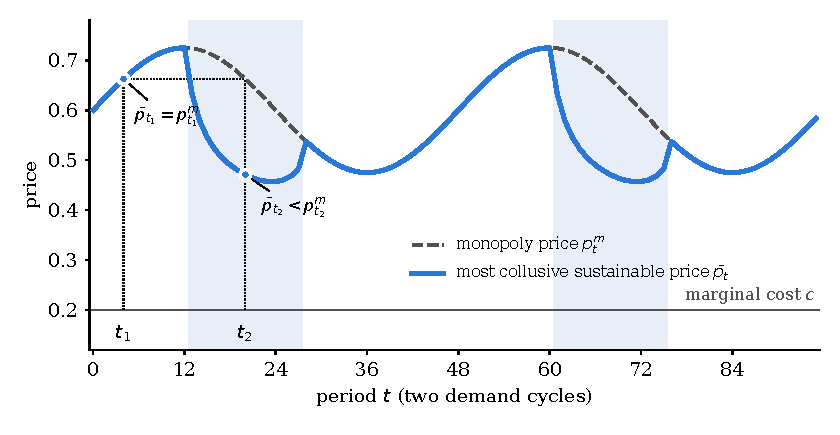
\includegraphics[width=0.92\textwidth]{figures/ch13/bs_cycle.pdf}
\caption{Most collusive sustainable price over a deterministic demand cycle. Linear demand
$D_t(p)=a_t-p$ with $a_t=1+0.25\sin\left(\frac{2\pi t}{48}\right)$, marginal cost $c=0.2$, $N=8$ firms,
$\delta=0.99$ per period and a ten-period Bertrand punishment. Shaded periods are those in which the
incentive constraint \eqref{eq:13-gas-ic} binds. Demand is the same at $t_1$ (rising) and $t_2$ (falling),
yet $\bar p_{t_1}=p^m_{t_1}=0.66$ while $\bar p_{t_2}=0.47$. The path solves \eqref{eq:13-gas-fixed} by
iteration (script \texttt{bs\_cycle.py}).}
\label{fig:13-bs-cycle}
\end{figure}

\casehead{From the incentive constraint to a margin regression}
To motivate an estimating equation we linearize the binding constraint. Let $M_t=\bar p_t-c_t$ be the
collusive margin, $L_t=\frac{M_t}{\bar p_t}$ the Lerner index (a local use of $L_t$, which denotes the lakes
dummy in \cref{sec:13-jec}), and
$\varepsilon_t=-\frac{d'(\bar p_t)\bar p_t}{d(\bar p_t)}$ the industry demand elasticity. At a binding date,
taking logs of $(N-1)A_tM_td(c_t+M_t)=\Phi_t$ gives
\begin{equation*}
\ln A_t+\ln M_t+\ln d(c_t+M_t)=\ln\Phi_t-\ln(N-1).
\end{equation*}
Differentiate, using $\frac{d'}{d}=-\frac{\varepsilon_t}{\bar p_t}$:
\begin{equation*}
\Big(\frac{1}{M_t}-\frac{\varepsilon_t}{\bar p_t}\Big)\,\dd M_t=\dd\ln\Phi_t-\dd\ln A_t+\frac{\varepsilon_t}{\bar p_t}\,\dd c_t .
\end{equation*}
The bracket equals $\frac{1-\varepsilon_tL_t}{M_t}$. It is positive below the monopoly price, because there
profit rises with price: $\frac{\dd}{\dd p}\big[(p-c_t)d(p)\big]=d(p)\,(1-\varepsilon_tL_t)>0$. Near a stationary
point the weights
$\omega_s=\frac{\delta^s}{\sum_{r=1}^{T}\delta^r}$ give $\dd\ln\Phi_t=\sum_s\omega_s\,\dd\ln\bar v_{t+s}$. Hold
future margins at their stationary values, so that future profits move only through demand and cost:
$\dd\ln\bar v_{t+s}=\dd\ln A_{t+s}-\frac{\varepsilon}{\bar p}\dd c_{t+s}$. Substituting and collecting terms,
\begin{equation}\label{eq:13-gas-linear}
\dd M_t=\frac{M}{1-\varepsilon L}\sum_{s=1}^{T}\omega_s\big(\dd\ln A_{t+s}-\dd\ln A_t\big)
-\frac{\varepsilon L}{1-\varepsilon L}\sum_{s=1}^{T}\omega_s\big(\dd c_{t+s}-\dd c_t\big).
\end{equation}
The current levels of demand and cost enter only through their expected changes. With a one-period horizon
and expectations formed at $t$, the margin equation becomes
\begin{equation}\label{eq:13-gas-reg}
M_t\approx\alpha_0+\alpha_2\,\E_t\big[\Delta\ln A_{t+1}\big]+\alpha_3\,\E_t\big[\Delta c_{t+1}\big],\qquad
\alpha_2=\frac{M}{1-\varepsilon L}>0,\quad \alpha_3=-\frac{\varepsilon L}{1-\varepsilon L}<0 .
\end{equation}
The coefficients $\alpha_2$ and $\alpha_3$ are local to this section and have nothing to do with the logit
price coefficient. Under the static benchmark of \cref{prop:13-gas-cs}(c), $\alpha_2=\alpha_3=0$. This is
the null hypothesis that \citet{BorensteinShepard1996} test.

If punishments last longer than one period, the one-period expected change is only a proxy for the weighted
change in \eqref{eq:13-gas-linear}. Under the static null the margin responds to neither, so the proxy
coefficients are still zero and the test keeps its size. Under the alternative the direction of the bias is not
determined. Take demand, and let $\Delta^{1}_t = \E_t[\Delta\ln A_{t+1}]$ and
$\Delta^{T}_t = \sum_{s=1}^{T}\omega_s\E_t[\ln A_{t+s} - \ln A_t]$, both residualized on the other regressors.
Since the weights sum to one, $\Delta^{T}_t = \Delta^{1}_t + R_t$, with $R_t$ the residual of
$\sum_{s=2}^{T}\omega_s\E_t[\ln A_{t+s} - \ln A_{t+1}]$ on the other regressors. Ignoring the cross effect through the cost proxy, the
coefficient on $\Delta^{1}_t$ converges to
\begin{equation*}
\alpha_2\,\frac{\Cov(\Delta^{1}_t, \Delta^{T}_t)}{\Var(\Delta^{1}_t)}
= \alpha_2\left[1 + \frac{\Cov(\Delta^{1}_t, R_t)}{\Var(\Delta^{1}_t)}\right] .
\end{equation*}
The estimate is attenuated only if later expected changes are negatively correlated with the next one, and not so
strongly that the sign reverses. On a smooth seasonal cycle with a horizon of a few months, expected changes in
consecutive months tend to share a sign. The ratio then exceeds one, and the estimate overstates $\alpha_2$. The
same argument applies to $\alpha_3$.

\begin{remark}[Why level and change can be separated]\label{rem:13-gas-level-change}
With independent draws, $\E_t[\ln A_{t+1}]$ is a constant, so $\E_t[\Delta\ln A_{t+1}]=\text{const}-\ln A_t$.
The level of demand and its expected change are then perfectly collinear, and a high level always signals
an expected fall. A seasonal cycle breaks the collinearity. Two weeks with the same demand, one before and
one after the seasonal peak, have opposite expected changes. That is why the test needs predictable
movements in demand and cost.
\end{remark}

\casehead{Competing explanations and the sign of the cost effect}
Two non-collusive mechanisms could also tie current margins to expected future conditions. Both predict
the opposite sign for the cost effect. The first is inventories. Suppose a supplier prices off its
replacement cost, the terminal price $w_{t+1}$ expected at its next purchase, and adds a constant margin
$m^{\circ}$. Then $p_t=\E_t[w_{t+1}]+m^{\circ}$, and the observed margin is
\begin{equation}\label{eq:13-gas-inventory}
M_t=p_t-w_t=m^{\circ}+\E_t\big[\Delta w_{t+1}\big].
\end{equation}
The coefficient on the expected cost change is $+1$, while collusion predicts $\alpha_3<0$. The second
mechanism is a cost of changing prices. A firm facing such costs moves its price toward the price it expects
to want in the future. An anticipated cost increase then raises today's price and today's margin, again a
positive sign. A negative coefficient on expected cost changes is therefore a distinctive prediction of
dynamic collusion. Inventory motives tied to demand require a risk of stockouts, which
\citet{BorensteinShepard1996} rule out because wholesale purchases were never constrained in their sample.

\subsection{Margins and expected demand in U.S.\ cities: Borenstein and Shepard (1996)}\label{sec:13-bs}

\casehead{Question}
Earlier tests of collusion used contemporaneous prices, quantities and costs, as in the conduct-parameter
studies of \cref{ch:conduct}. \citet{Bresnahan1989} stressed that such tests rest on functional-form
assumptions, because static non-cooperative prices can move either way with demand. \citet{BorensteinShepard1996}
ask whether current retail gasoline margins respond to \emph{expected} changes in demand and wholesale cost.
Under static pricing they should not respond at all, so a response is evidence of dynamic collusion that
does not depend on the shape of demand or cost. The question matters because gasoline retailing is far from
a tight oligopoly. Most metropolitan areas have more than ten wholesale suppliers and many more stations.

\casehead{Setting}
Crude oil is refined and shipped by pipeline or barge to city terminals. From the terminal, gasoline is
trucked to stations either by independent wholesalers, called \emph{jobbers}, or by refiners. Jobbers
distribute about 55 percent of U.S. retail gasoline and pay the posted terminal price
(working paper, pp.~8--10). Refiners sell to independently operated stations at the \emph{dealer tankwagon}
price, which is subject to widespread unobserved discounts. Borenstein and Shepard therefore measure
marginal cost by the terminal price. It is the only observed wholesale price for jobbers, it is the
opportunity cost of gasoline sold at refiner-supplied stations, and it is rarely discounted. The margin they
study is the gap between the retail price and the terminal price. It mixes decisions of refiners, jobbers and
station operators.

\casehead{Data}
The panel covers 59 cities in 43 states over the 72 months from 1986 to 1991. \textit{RETAIL} is the Lundberg
Survey average price of regular unleaded self-service gasoline, net of all taxes, on one Friday each month.
\textit{TERM} is the average branded terminal price posted on the same Friday, so the two prices match exactly
and $\textit{MARGIN}=\textit{RETAIL}-\textit{TERM}$. Volume comes from monthly state sales reported by the
Federal Highway Administration. Daily volume in adjacent months is interpolated linearly to the survey day,
giving \textit{VOLUME}. Because over 99 percent of the variance of \textit{VOLUME} is between states,
volume is normalized by its state mean: $\textit{NVOLUME}_{it}=\frac{\textit{VOLUME}_{it}}{\overline{\textit{VOLUME}}_i}$.
\Cref{tab:13-bs-t1} reports the summary statistics. Demand peaks in August at about 20 percent above the
January trough. Short-run demand elasticities lie between $-0.1$ and $-0.2$ \citep{DahlSterner1991}. Retail
prices would then have to swing by 100--200 percent to generate such a cycle, so the seasonal pattern reflects
shifts of demand rather than movements along it. Over half of the monthly crude oil price changes exceed 5
percent in absolute value.

\begin{table}[htbp]
\centering
\caption{Retail gasoline in 59 U.S. cities, 1986--1991: summary statistics}\label{tab:13-bs-t1}
\begin{tabular}{lrrrr}
\toprule
Variable & Mean & Std.\ dev. & Min & Max\\
\midrule
\textit{RETAIL} (cents per gallon) & 72.83 & 12.41 & 43.18 & 126.57\\
\textit{TERM} (cents per gallon) & 62.28 & 11.82 & 36.00 & 111.88\\
\textit{CRUDE} (cents per gallon) & 46.38 & 10.77 & 25.83 & 87.98\\
\textit{MARGIN} (cents per gallon) & 10.57 & 5.12 & $-8.91$ & 34.90\\
\textit{VOLUME} ($10^5$ or $10^6$ gallons per day, see notes) & 10.43 & 10.48 & 0.38 & 38.12\\
\textit{NVOLUME} & 1.005 & 0.087 & 0.570 & 1.617\\
\textit{EXP VOLCHG}, $\hat\eta=-0.1$ & 0.000 & 0.050 & $-0.403$ & 0.287\\
\textit{EXP TERMCHG} (cents per gallon) & 0.139 & 4.172 & $-17.313$ & 13.959\\
\bottomrule
\end{tabular}

\smallskip
\begin{minipage}{0.86\textwidth}\footnotesize
Notes: 3,838 city-month observations. Prices exclude sales and excise taxes and are in current cents.
\textit{EXP VOLCHG} and \textit{EXP TERMCHG} are the expected one-month changes in normalized volume and in the
terminal price defined in the text. The unit of \textit{VOLUME} is unclear in the sources. The working paper's Table 1
prints it as ``(00,000 gal/day)'' and the published Table 1 as gallons $\times 10^{5}$ per day (p.~434). The volume figures
of both versions label the same daily state series in millions of gallons, at levels close to the table means (published
Figure 2, p.~437). We report the numbers as printed and leave the unit open. \textit{NVOLUME} and the regressions do not
depend on it. Source: \citet{BorensteinShepard1996}, working-paper version, Table 1.
\end{minipage}
\end{table}

\casehead{The estimating equation}
Retail prices adjust to terminal prices with lags, and increases pass through faster than decreases. The
authors start from an error-correction model with asymmetric adjustment (working paper, eq.~(1)):
\begin{equation}\label{eq:13-bs-ecm}
\begin{aligned}
\textit{RETAIL}_{it}-\textit{RETAIL}_{i,t-1}={}&\beta_1\Delta\textit{TERM}^{+}_{it}+\beta_2\Delta\textit{TERM}^{+}_{i,t-1}+\beta_3\Delta\textit{TERM}^{+}_{i,t-2}\\
&+\beta_4\Delta\textit{TERM}^{-}_{it}+\beta_5\Delta\textit{TERM}^{-}_{i,t-1}+\beta_6\Delta\textit{TERM}^{-}_{i,t-2}\\
&+\beta_7\Delta\textit{RETAIL}^{+}_{i,t-1}+\beta_8\Delta\textit{RETAIL}^{+}_{i,t-2}\\
&+\beta_9\Delta\textit{RETAIL}^{-}_{i,t-1}+\beta_{10}\Delta\textit{RETAIL}^{-}_{i,t-2}\\
&+\beta_{11}\textit{RETAIL}_{i,t-1}+\beta_{12}\textit{TERM}_{i,t-1}+e_{it}.
\end{aligned}
\end{equation}
Here $\Delta X_{it}=X_{it}-X_{i,t-1}$, and $\Delta X^{+}$ and $\Delta X^{-}$ are the positive and negative parts
of the change. The lagged levels form the error-correction term. If the long-run relation is
$\textit{RETAIL}=\gamma_0+\gamma_1\textit{TERM}$ and the gap closes at rate $\kappa>0$, the correction
$-\kappa(\textit{RETAIL}_{t-1}-\gamma_0-\gamma_1\textit{TERM}_{t-1})$ produces the two lagged levels, with
$\beta_{11}=-\kappa$ and $\beta_{12}=\kappa\gamma_1$. The constant is absorbed by fixed effects.

To put the margin on the left, add $\textit{RETAIL}_{i,t-1}$ to both sides and subtract $\textit{TERM}_{it}$.
The left side becomes $\textit{MARGIN}_{it}$. On the right, $\textit{TERM}_{it}=\Delta\textit{TERM}^{+}_{it}+
\Delta\textit{TERM}^{-}_{it}+\textit{TERM}_{i,t-1}$, so subtracting it lowers the coefficients on
$\Delta\textit{TERM}^{+}_{it}$ and $\Delta\textit{TERM}^{-}_{it}$ by one and the coefficient on
$\textit{TERM}_{i,t-1}$ by one. Adding $\textit{RETAIL}_{i,t-1}$ raises its coefficient by one. The margin
form (working paper, eq.~(2)) is therefore \eqref{eq:13-bs-ecm} with $\beta_1-1$, $\beta_4-1$, $\beta_{11}+1$
and $\beta_{12}-1$ in place of $\beta_1$, $\beta_4$, $\beta_{11}$ and $\beta_{12}$. Adding current volume and the
two expectation terms gives the estimating equation (working paper, eq.~(3)), in which the coefficient
adjustments are left implicit:
\begin{equation}\label{eq:13-bs-main}
\begin{aligned}
\textit{MARGIN}_{it}={}&\alpha_1\textit{NVOLUME}_{it}+\alpha_2\textit{EXP VOLCHG}_{it}+\alpha_3\textit{EXP TERMCHG}_{it}\\
&+\sum_{k=0}^{2}\big(\beta^{+}_{k}\Delta\textit{TERM}^{+}_{i,t-k}+\beta^{-}_{k}\Delta\textit{TERM}^{-}_{i,t-k}\big)\\
&+\sum_{k=1}^{2}\big(\phi^{+}_{k}\Delta\textit{RETAIL}^{+}_{i,t-k}+\phi^{-}_{k}\Delta\textit{RETAIL}^{-}_{i,t-k}\big)\\
&+\beta_{11}\textit{RETAIL}_{i,t-1}+\beta_{12}\textit{TERM}_{i,t-1}+\mu_i+\lambda_t+e_{it}.
\end{aligned}
\end{equation}
We have relabeled the twelve $\beta$'s of the original to show the pattern. The terms $\mu_i$ and
$\lambda_t$ (local symbols here) are city fixed effects and 72 month fixed effects, which absorb cross-city correlation of the
errors at a point in time. Current volume $\alpha_1$ captures any static effect of demand on margins, such as
changes in the mix of customers or peak-load pricing. The coefficients of interest are $\alpha_2$ and
$\alpha_3$, the empirical counterparts of \eqref{eq:13-gas-reg}. The effect of current volume holding expected
next-month volume fixed is $\alpha_1-\alpha_2$, because $\textit{EXP VOLCHG}$ is expected next-month volume
minus current volume.

\casehead{Endogeneity of volume: an instrument built from an assumed elasticity}
Volume depends on the retail price and hence on the margin, so OLS is inconsistent, and no excluded demand
shifters are available. The authors resolve the problem with a constructed instrument. Write the system
(working paper, eqs.~(4) and~(5))
\begin{equation}\label{eq:13-bs-system}
M=a\,Q+X^{\top}g+e,\qquad \ln Q=Z\beta+\eta\ln P+v.
\end{equation}
Here $M$ is the margin, $Q$ volume, $P$ the retail price and $X$ the exogenous variables in the margin
equation. $Z$ collects demand shifters, $\eta<0$ is the industry demand elasticity, and $e$ and $v$ are errors.
The working paper assumes only that $e$ and $v$ are uncorrelated. We assume instead that the margin error is mean
independent of the exogenous variables and of the demand shock, $\E[e\mid X,Z,v]=0$. If $\eta$ were known, the
variable
\begin{equation}\label{eq:13-bs-qprime}
\ln Q'=\ln Q+\ln k-\eta\ln P=Z\beta+\ln k+v
\end{equation}
would be volume purged of the direct price effect. It is a function of $Z$ and $v$ only. Mean independence
therefore makes it, and any function of it, uncorrelated with $e$. It is correlated with $Q$, so it is a valid
instrument. The stronger condition matters because the instrument used below is the level $Q'$, which is
proportional to $\exp(v)$ given $Z$. Uncorrelatedness does not carry over to the level. If $v$ is uniform on
$\{-1,0,1\}$ and $e=v^2-\frac{2}{3}$, then $\E[e]=\E[ev]=0$ but
$\E[e\exp(v)]=\frac{\exp(1)+\exp(-1)-2}{9}>0$. Some demand shifters may themselves respond to
$P$, for example prices of other goods that rise with transport costs. Partition $Z=(Z_1,Z_2)$ with
$Z_1=\theta_0+\theta_1\ln P$ and $Z_2$ independent of $P$. Then
\begin{equation*}
\ln Q=(\theta_0+\theta_1\ln P)\beta_1+Z_2\beta_2+\eta\ln P+v,
\end{equation*}
and the variable
\begin{equation}\label{eq:13-bs-qdoubleprime}
\ln Q''=\ln Q+\ln k-\tilde\eta\ln P=\theta_0\beta_1+Z_2\beta_2+\ln k+v,\qquad \tilde\eta\equiv\eta+\theta_1\beta_1,
\end{equation}
is again a valid instrument if $\E[e\mid X,Z_2,v]=0$. Published estimates of gasoline demand elasticities ignore such indirect effects,
so they are best read as estimates of $\tilde\eta$.

The implementation multiplies daily volume by $kP^{-\hat\eta}$ with $k=\frac{\bar P^{\hat\eta}}{\bar Q}$,
where $\bar P$ is the city's mean retail price and $\bar Q$ the mean of the corrected series. The result,
$\textit{TNVOLUME}=\frac{\textit{VOLUME}}{\bar Q}\left(\frac{P}{\bar P}\right)^{-\hat\eta}$, instruments
\textit{NVOLUME} in two-stage least squares. Since $\hat\eta$ is unknown, the regression is repeated for
$\hat\eta\in\{0,-0.1,-0.2,-0.3\}$, a range slightly wider than the $-0.1$ to $-0.2$ found with monthly and
quarterly data. With $\hat\eta=0$ the correction is void and \textit{NVOLUME} is treated as exogenous. The
correction is small: a price 20 percent above the city mean raises \textit{TNVOLUME} relative to
\textit{NVOLUME} by $1.2^{0.3}-1=5.6$ percent when $\hat\eta=-0.3$ and by $1.2^{0.1}-1=1.8$ percent when
$\hat\eta=-0.1$.

The contemporaneous terminal price could also be endogenous if the marginal cost of supplying a city rises
with its volume. The authors argue that the feedback is small, because terminals have ten or more refiners
and supply can shift across regions. A Hausman test nonetheless rejects exogeneity of the current terminal
price and of the expected terminal-price change. The current price is therefore instrumented with the residual
from a regression of \textit{TERM} on \textit{NVOLUME}. The expected change is instrumented with a forecast built
from that orthogonalized series. Instrumenting does not change the results in an economically or statistically
meaningful way. The residuals of \eqref{eq:13-bs-main}
are not serially correlated, so the lagged dependent variables raise no endogeneity problem.

\casehead{Measuring expectations}
Expected volume comes from a forecasting regression estimated state by state (working paper, eq.~(8)):
\begin{equation}\label{eq:13-bs-volforecast}
\textit{NVOLUME}_{it}=a_0+a_1\textit{NVOLUME}_{i,t-1}+a_2\textit{NVOLUME}_{i,t-2}+\sum_{j=2}^{12}\varsigma_j\textit{MONTH}_j
+a_3t+a_4t^2+a_5t^3+e_{it}.
\end{equation}
The $R^2$ lies between 0.80 and 0.95 for nearly all states. The one-period lead of the fitted values gives
$\textit{EXP VOLCHG}_{it}=\widehat{\textit{NVOLUME}}_{i,t+1}-\textit{NVOLUME}_{it}$. The instrument for
\textit{EXP VOLCHG} uses the same regression estimated with \textit{TNVOLUME}. Expected terminal prices come
from a city-level error-correction autoregression with crude oil prices (working paper, eq.~(9)):
\begin{equation}\label{eq:13-bs-termforecast}
\begin{aligned}
\Delta\textit{TERM}_{it}={}&b_0+\sum_{k=1}^{2}\big(b^{+}_k\Delta\textit{TERM}^{+}_{i,t-k}+b^{-}_k\Delta\textit{TERM}^{-}_{i,t-k}
+d^{+}_k\Delta\textit{CRUDE}^{+}_{i,t-k}+d^{-}_k\Delta\textit{CRUDE}^{-}_{i,t-k}\big)\\
&+b_9\textit{TERM}_{i,t-1}+b_{10}\textit{CRUDE}_{i,t-1}+\sum_{j=2}^{12}\varsigma'_j\textit{MONTH}_j+e_{it}.
\end{aligned}
\end{equation}
The current crude price is excluded because it would not be known when the forecast is made. The $R^2$ ranges
from 0.30 to 0.60, lower than for volume because crude prices behave roughly like a random walk. Then
$\textit{EXP TERMCHG}_{it}=\widehat{\Delta\textit{TERM}}_{i,t+1}$. The forecasting coefficients use the whole
sample, which in principle includes information the firms did not have. Forecasts from rolling regressions
with volume data back to 1982 change neither the predictions nor the final coefficients substantively.

\casehead{Identification}
The month fixed effects absorb any national seasonal pattern, including the common August peak. The
coefficient on \textit{EXP VOLCHG} is therefore identified from differences in seasonal patterns across states
and from state-specific trends. These differences are large. The peak-to-trough swing is 51 percent of mean
volume in Wyoming and 7 percent in Arizona. August demand is below the state mean in Florida, and January
demand is above it in Colorado and Hawaii (working paper, p.~27). The coefficient on \textit{EXP TERMCHG} is
identified from city-specific terminal-price dynamics. Cold-weather cities, for instance, see winter declines
in gasoline terminal prices when refiners produce heating oil and gasoline jointly. The expectation terms are
functions of lagged variables and deterministic seasonals, so they are predetermined with respect to the
current margin shock.

\casehead{Results}
\Cref{tab:13-bs-t2} reproduces the two-stage least squares estimates. The coefficient on \textit{EXP VOLCHG} is
positive and significant at the 1 percent level for every assumed elasticity, and it changes little with
$\hat\eta$. The coefficient on \textit{EXP TERMCHG} is negative and significant at the 1 percent level
throughout. Both signs are those of \eqref{eq:13-gas-reg}. The negative cost coefficient is the opposite of the
inventory prediction \eqref{eq:13-gas-inventory}.

\begin{table}[htbp]
\centering
\caption{Retail margins and expected changes in demand and cost (dependent variable \textit{MARGIN})}\label{tab:13-bs-t2}
\small
\begin{tabular}{lcccc}
\toprule
Assumed elasticity & $\hat\eta=0$ & $\hat\eta=-0.1$ & $\hat\eta=-0.2$ & $\hat\eta=-0.3$\\
\midrule
$\textit{NVOLUME}_t$ & 3.397 (0.754) & 5.563 (0.758) & 7.926 (0.768) & 10.455 (0.785)\\
$\textit{EXP VOLCHG}_t$ & 4.081 (1.324) & 3.860 (1.335) & 4.362 (1.365) & 5.492 (1.409)\\
$\textit{EXP TERMCHG}_t$ & $-0.057$ (0.018) & $-0.062$ (0.017) & $-0.066$ (0.018) & $-0.068$ (0.018)\\
\addlinespace
$\Delta\textit{TERM}^{+}_t$ & $-0.303$ (0.021) & $-0.305$ (0.021) & $-0.306$ (0.021) & $-0.304$ (0.021)\\
$\Delta\textit{TERM}^{+}_{t-1}$ & 0.153 (0.023) & 0.148 (0.023) & 0.143 (0.023) & 0.138 (0.023)\\
$\Delta\textit{TERM}^{+}_{t-2}$ & 0.065 (0.021) & 0.063 (0.021) & 0.062 (0.021) & 0.061 (0.022)\\
$\Delta\textit{TERM}^{-}_t$ & $-0.589$ (0.019) & $-0.584$ (0.019) & $-0.578$ (0.019) & $-0.572$ (0.018)\\
$\Delta\textit{TERM}^{-}_{t-1}$ & 0.175 (0.023) & 0.169 (0.023) & 0.163 (0.023) & 0.155 (0.023)\\
$\Delta\textit{TERM}^{-}_{t-2}$ & 0.078 (0.020) & 0.074 (0.020) & 0.069 (0.020) & 0.065 (0.020)\\
$\Delta\textit{RETAIL}^{+}_{t-1}$ & $-0.017$ (0.022) & $-0.018$ (0.023) & $-0.020$ (0.023) & $-0.022$ (0.023)\\
$\Delta\textit{RETAIL}^{+}_{t-2}$ & $-0.066$ (0.022) & $-0.069$ (0.022) & $-0.072$ (0.022) & $-0.076$ (0.022)\\
$\Delta\textit{RETAIL}^{-}_{t-1}$ & $-0.029$ (0.022) & $-0.027$ (0.022) & $-0.026$ (0.023) & $-0.025$ (0.023)\\
$\Delta\textit{RETAIL}^{-}_{t-2}$ & 0.039 (0.020) & 0.039 (0.020) & 0.039 (0.020) & 0.039 (0.020)\\
$\textit{RETAIL}_{t-1}$ & 0.623 (0.015) & 0.619 (0.015) & 0.615 (0.015) & 0.612 (0.015)\\
$\textit{TERM}_{t-1}$ & $-0.668$ (0.020) & $-0.660$ (0.020) & $-0.650$ (0.020) & $-0.639$ (0.020)\\
\addlinespace
Observations & 3,838 & 3,838 & 3,838 & 3,838\\
\bottomrule
\end{tabular}

\smallskip
\begin{minipage}{0.92\textwidth}\footnotesize
Notes: Two-stage least squares estimates of \eqref{eq:13-bs-main} with city and month fixed effects (not
reported). Asymptotic standard errors in parentheses. \textit{NVOLUME} is instrumented with the
elasticity-corrected series for the assumed $\hat\eta$. Source: \citet{BorensteinShepard1996}, working-paper
version, Table 2.
\end{minipage}
\end{table}

\begin{example}[Reading the magnitudes]\label{ex:13-bs-elasticity}
Take the column $\hat\eta=-0.1$, which the authors regard as closest to the true elasticity. Raise expected
next-month volume by 1 percent of its mean, that is by $0.01005$ units of \textit{NVOLUME}, holding current
volume fixed. \textit{EXP VOLCHG} rises by the same amount, so the margin rises by $3.860\times0.01005=0.039$
cents, which is $\frac{0.039}{10.57}=0.37$ percent of the mean margin. The elasticity of the margin with respect
to expected next-month volume is therefore 0.37. Raise the expected next-month terminal price by 1 percent of its
mean, or 0.623 cents. The margin falls by $0.062\times0.623=0.039$ cents, an elasticity of $-0.37$. These are the
two elasticities in the authors' abstract. A one-standard-deviation increase in \textit{EXP VOLCHG} (0.050) adds
$3.860\times0.050=0.19$ cents to the margin. A one-standard-deviation increase in \textit{EXP TERMCHG} (4.172
cents) subtracts $0.062\times4.172=0.26$ cents.

The seasonal peak shows how the two volume terms combine. July volume averages 8.3 percent above the sample
mean, which adds $5.563\times0.083=0.46$ cents to the July margin. August volume is 8.8 percent above the mean,
so the expected July-to-August change of 0.5 percent adds $3.860\times0.005=0.02$ cents, for a total of 0.48 cents.
In August, current volume adds $5.563\times0.088=0.49$ cents. The expected fall of 4.6 percent into September
subtracts $3.860\times0.046=0.18$ cents, so August margins are only 0.31 cents above average. Margins are higher
on the way up to the peak than at the peak itself, as \cref{fig:13-bs-cycle} predicts.
\end{example}

The rest of the table describes price adjustment. A one-cent rise in the terminal price lowers the margin in
the same month by 0.305 cents, so the retail price rises by $1-0.305=0.70$ cents within the month. A one-cent
fall raises the margin by 0.584 cents, so the retail price falls by only $1-0.584=0.42$ cents. Increases pass
through faster than decreases. The long-run pass-through follows from the lagged levels. Setting all changes to
zero in \eqref{eq:13-bs-main} gives $\textit{RETAIL}(1-\beta_{11})=\textit{TERM}(1+\beta_{12})+\text{const}$, so
\begin{equation*}
\frac{\partial\,\textit{RETAIL}}{\partial\,\textit{TERM}}\bigg|_{\text{long run}}=\frac{1+\beta_{12}}{1-\beta_{11}}
=\frac{1-0.660}{1-0.619}=0.89 .
\end{equation*}
This matches the authors' statement that terminal price changes are passed through about 90 percent in the long
run, a rate they cannot distinguish statistically from 100 percent.

\begin{example}[How large should the effects be?]\label{ex:13-gas-calibration}
The linearized constraint \eqref{eq:13-gas-reg} gives a benchmark for the coefficients. Take the sample means
$M=10.57$ and $\bar p=72.83$ cents, so $L=0.145$, and an industry elasticity between 0.1 and 0.3. Then
$\varepsilon L$ lies between 0.015 and 0.044. The benchmark is $\alpha_2=\frac{M}{1-\varepsilon L}$, between 10.7
and 11.1 cents per unit change in $\ln A$, and $\alpha_3=-\frac{\varepsilon L}{1-\varepsilon L}$, between $-0.015$
and $-0.045$. The estimates of 3.86 and $-0.062$ are of the same order of magnitude. The comparison is only
indicative. The benchmark assumes that the constraint always binds, that punishments last one month, that the
whole measured margin is collusive and that future margins do not move.
\end{example}

\casehead{Robustness: expected versus unexpected changes}
The main threat is measurement error. Monthly state volumes are matched to a single day's city prices. If
current volume is measured with error and next month's volume contains information about current volume, then
\textit{EXP VOLCHG} could proxy for the true current volume. Since current volume raises margins, this would
mimic the collusive effect. The two explanations differ in their predictions for \emph{unexpected} future
changes. Firms cannot respond to changes they do not foresee, so under collusion unexpected changes have zero
coefficients. Under measurement error, unexpected changes would carry information about current volume as
well. The authors estimate (working paper, eq.~(3$'$))
\begin{equation}\label{eq:13-bs-unx}
\begin{aligned}
\textit{MARGIN}_{it}={}&\alpha_1\textit{EXP VOL}_{it}+\alpha'_1\textit{UNX VOL}_{it}+\alpha_2\textit{EXP VOLCHG}_{it}
+\alpha'_2\textit{UNX VOLCHG}_{it}\\
&+\alpha_3\textit{EXP TERMCHG}_{it}+\alpha'_3\textit{UNX TERMCHG}_{it}\\
&+(\text{price-adjustment terms and fixed effects of \eqref{eq:13-bs-main}})+e_{it}.
\end{aligned}
\end{equation}
Here $\textit{UNX VOLCHG}$ is next month's actual volume change minus its expected value. The terms
$\textit{EXP VOL}$ and $\textit{UNX VOL}$ split current volume into the part predicted a month earlier and the
surprise.
\Cref{tab:13-bs-t3} reports the key rows. Unexpected future volume changes are never significantly positive, and
they differ significantly from expected changes for every nonzero $\hat\eta$. Unexpected terminal changes have
coefficients near zero, significantly different from the expected ones. Unexpected \emph{current} volume
raises margins significantly for every nonzero $\hat\eta$. Margins therefore do respond to current surprises.
Their failure to respond to future surprises is informative.

\begin{table}[htbp]
\centering
\caption{Expected versus unexpected changes (dependent variable \textit{MARGIN})}\label{tab:13-bs-t3}
\small
\begin{tabular}{lcccc}
\toprule
Assumed elasticity & $\hat\eta=0$ & $\hat\eta=-0.1$ & $\hat\eta=-0.2$ & $\hat\eta=-0.3$\\
\midrule
$\textit{EXP NVOLUME}_t$ & 4.116 (0.824) & 5.150 (0.830) & 6.273 (0.846) & 7.478 (0.871)\\
$\textit{UNX NVOLUME}_t$ & 0.926 (1.388) & 7.003 (1.402) & 13.347 (1.447) & 19.751 (1.518)\\
$\textit{EXP VOLCHG}_t$ & 3.720 (1.334) & 4.064 (1.347) & 4.930 (1.382) & 6.129 (1.436)\\
$\textit{UNX VOLCHG}_t$ & 1.178 (1.292) & 0.146 (1.309) & $-1.478$ (1.355) & $-3.532$ (1.425)\\
$\textit{EXP TERMCHG}_t$ & $-0.059$ (0.018) & $-0.059$ (0.018) & $-0.057$ (0.018) & $-0.054$ (0.018)\\
$\textit{UNX TERMCHG}_t$ & 0.013 (0.016) & 0.011 (0.016) & 0.009 (0.016) & 0.006 (0.016)\\
\addlinespace
Observations & 3,838 & 3,838 & 3,838 & 3,838\\
\bottomrule
\end{tabular}

\smallskip
\begin{minipage}{0.92\textwidth}\footnotesize
Notes: Estimates of \eqref{eq:13-bs-unx}. The price-adjustment terms, city and month fixed effects are included
and not shown. Standard errors in parentheses. Source: \citet{BorensteinShepard1996}, working-paper version,
Table 3.
\end{minipage}
\end{table}

\casehead{Interpretation}
Borenstein and Shepard read the evidence as consistent with tacit collusion in the sense of
\citet{RotembergSaloner1986} and \citet{HaltiwangerHarrington1991}. They stress what the test does not show.
Collusion here need not mean prices near monopoly. With an industry elasticity between $-0.1$ and $-0.3$, demand
is inelastic at observed prices, so an industry monopolist would raise prices far above them. The authors conclude
that actual margins fall far short of the monopoly level. Nor does the test measure the level of collusion. The
measured margin includes delivery and other short-run variable costs, so the collusive part is smaller than 10.6
cents, and the data cannot isolate it. What the test detects is the dynamic signature of an incentive constraint.
A mild form of tacit coordination fits the market: a station that cuts
its price provokes nearby stations to retaliate, and the retaliation is costlier when future margins are high.

\casehead{Critiques}
Five limitations deserve mention. First, expectations are the econometrician's forecasts. Their coefficients are
estimated on the full sample, and the true information sets of station managers are unknown. Second, volume is
measured at the state level, prices at the city level, and prices only on one day per month. Third, the
one-month horizon is arbitrary. The authors argue that longer punishments would bias the estimates downward
(working paper, p.~17). That holds only under the covariance condition stated after \eqref{eq:13-gas-reg}, and on
a seasonal cycle the bias can go either way. The test of the static null keeps its size in either case. Fourth, the test rejects static pricing, but other dynamic
non-cooperative models could generate forward-looking prices. \Cref{sec:13-noel} shows that Edgeworth cycles are one
such model, although its mechanism differs from the one tested here. Fifth, the margin mixes the decisions of
refiners, jobbers and station operators, so the colluding agents are not identified.

\casehead{Contribution}
The paper moved the empirical study of collusion from tight oligopolies to an unconcentrated industry with many
differentiated sellers. It replaced contemporaneous price-cost relations, which require functional-form
assumptions, with a dynamic implication of the incentive constraint. It also showed how to build a test that
distinguishes collusion from inventory behavior and from measurement error through sign restrictions and a
placebo on unforecastable changes.

\subsection{Edgeworth cycles in Toronto: Noel (2007)}\label{sec:13-noel}

\casehead{Question}
In many Canadian cities retail gasoline prices follow a fast asymmetric cycle. A large, sudden price increase is
followed by many small decreases until margins are thin, and then prices jump again. Consumer groups and
governments have often read the synchronized jumps as collusion. \citet{Noel2007} asks whether the cycle is
instead a competitive \emph{Edgeworth cycle}, the Markov equilibrium of dynamic price competition introduced by
\citet{MaskinTirole1988}. The answer matters for policy, because evidence of Edgeworth cycles argues against
costly investigations of covert collusion.

\casehead{Theory}
In the model of \citet{MaskinTirole1988}, two firms sell a homogeneous good and set prices alternately, each price
fixed for two periods. Strategies are Markov: the moving firm conditions only on the rival's current price (and,
in the extension of \citet{Noel2007}, on the current cost). With demand $D^i$ for firm $i$ and cost $c_t$, firm
$i$ earns $\pi^i_t(p^1_t,p^2_t,c_t)=D^i(p^1_t,p^2_t)(p^i_t-c_t)$. When firm 1 moves after firm 2 has set
$p^2_{t-1}$, its values are
\begin{align}
V^1(p^2_{t-1})&=\E_c\Big[\max_{p_t}\big\{\pi^1_t(p_t,p^2_{t-1},c_t)+\delta_1W^1(p_t)\big\}\Big],\label{eq:13-mt-v}\\
W^1(p^1_{s-1})&=\E_c\Big[\E_{p_s}\big[\pi^1_s(p^1_{s-1},p_s,c_s)+\delta_1V^1(p_s)\big]\Big].\label{eq:13-mt-w}
\end{align}
Here $W^1$ is firm 1's value in a period in which firm 2 moves, and $p_s$ is firm 2's reply. The game has two
kinds of Markov perfect equilibria, focal-price equilibria and Edgeworth-cycle equilibria. The incentives
behind a cycle are as follows. At a high rival price, undercutting by one step captures the whole market for a
period, roughly twice what matching yields. Prices therefore fall step by step in the \emph{undercutting phase}.
Near marginal cost an undercut earns nothing. Raising the price is costly for the firm that moves first, because
the rival keeps the low price and serves the market for a period. Each firm prefers the other to restore prices,
so the bottom of the cycle is a war of attrition in which firms randomize between staying low and jumping up. The
firm that moves jumps all the way to the top in a single \emph{relenting phase}. A gradual increase would be
undercut at once and would not repay its cost. \Cref{fig:13-edgeworth} draws the resulting sawtooth.

\begin{figure}[htbp]
\centering
\begin{tikzpicture}
\begin{axis}[
  width=0.92\textwidth, height=6.4cm,
  xmin=-0.5, xmax=25, ymin=-0.9, ymax=12.6, clip=false,
  axis lines=left, xtick=\empty, ytick={2}, yticklabels={$c$},
  xlabel={period $t$ (firms move alternately)}, ylabel={price},
  legend style={draw=none, at={(0.5,-0.2)}, anchor=north, font=\footnotesize, legend columns=3,
    /tikz/every even column/.append style={column sep=0.6cm}},
  legend cell align=left,
]
\addplot[const plot, line width=1.6pt, orange!85!black] coordinates {
 (0,2) (1,9) (2,9) (3,7) (4,7) (5,5) (6,5) (7,3) (8,3) (9,2) (10,2) (11,10) (12,10) (13,8)
 (14,8) (15,6) (16,6) (17,4) (18,4) (19,2) (20,2) (21,2) (22,2) (23,9) (24,9) (25,9)};
\addlegendentry{firm 2 (moves at odd $t$)}
\addplot[const plot, line width=0.8pt, blue!70!black] coordinates {
 (0,10) (1,10) (2,8) (3,8) (4,6) (5,6) (6,4) (7,4) (8,2) (9,2) (10,2) (11,2) (12,9) (13,9)
 (14,7) (15,7) (16,5) (17,5) (18,3) (19,3) (20,2) (21,2) (22,10) (23,10) (24,8) (25,8)};
\addlegendentry{firm 1 (moves at even $t$)}
\addplot[dashed, gray, domain=-0.5:25] {2};
\addlegendentry{marginal cost $c$}
\draw[decorate, decoration={brace, amplitude=5pt}] (axis cs:1,10.7) -- (axis cs:9,10.7)
  node[midway, above=6pt, font=\footnotesize] {undercutting phase};
\draw[decorate, decoration={brace, amplitude=5pt, mirror}] (axis cs:8,1.3) -- (axis cs:11,1.3)
  node[midway, below=6pt, font=\footnotesize] {war of attrition};
\draw[-{Stealth[length=2mm]}] (axis cs:13.2,11.6) -- (axis cs:11.2,10.4);
\node[font=\footnotesize, anchor=west] at (axis cs:13.2,11.6) {relenting phase};
\end{axis}
\end{tikzpicture}
\caption{A stylized Edgeworth cycle with two symmetric firms. Each firm's price is fixed for two periods and firms
move in turn. Prices fall by one step per move until they reach marginal cost $c$. After a war of attrition one firm
relents to the top in a single jump, the rival undercuts it at once, and the cycle restarts. Where the two prices
coincide, the thin line lies on the thick one. Drawn by us after the logic of \citet{MaskinTirole1988} and Figure 2
of \citet{Noel2007}.}
\label{fig:13-edgeworth}
\end{figure}

Firm asymmetries sharpen the predictions. \citet{Eckert2003} lets firms split the market unequally at equal
prices. The firm with the smaller share at equal prices gains more from undercutting, since it gives up less of
the shared market, so small firms lead prices down. Large firms, which control many stations and coordinate them
easily, are better placed to restart the cycle. The theory thus makes one structural prediction and three
behavioral ones. The structural prediction is that each station raises its price by the full height of the cycle
in one period and then lowers it in small consecutive steps. The behavioral predictions are (1) fast but not
simultaneous reactions, (2) small firms lead prices down, and (3) large firms lead prices up. Edgeworth cycles
survive cost fluctuations and mild spatial differentiation, so the predictions carry over to retail gasoline.

\casehead{Data}
Noel collected retail prices every twelve hours at 22 Toronto stations on major routes over 131 consecutive days,
February 12 to June 22, 2001. Thirteen stations belong to major integrated firms and nine to independents, twelve
firms in all, spread over 17 miles. The price is for regular unleaded self-service gasoline in Canadian cents per
liter (cpl). The rack price is the daily spot price of the largest wholesaler at the Toronto rack, which can be
treated as exogenous because U.S. wholesale supply is readily available. Excise taxes are 24.7 cpl and the sales
tax is 7 percent. The average price before tax is 43.09 cpl (standard deviation 4.44), and after tax 72.53 (4.75).
The rack price averages 39.77 (4.00). The lagged retail price exceeds the rack price by 3.31 cpl (2.08) on
average (Table I). \Cref{fig:13-noel-f1} shows a major and an independent
station against the rack price. The retail cycle is evident, and the rack price has none.

\begin{figure}[htbp]
\centering
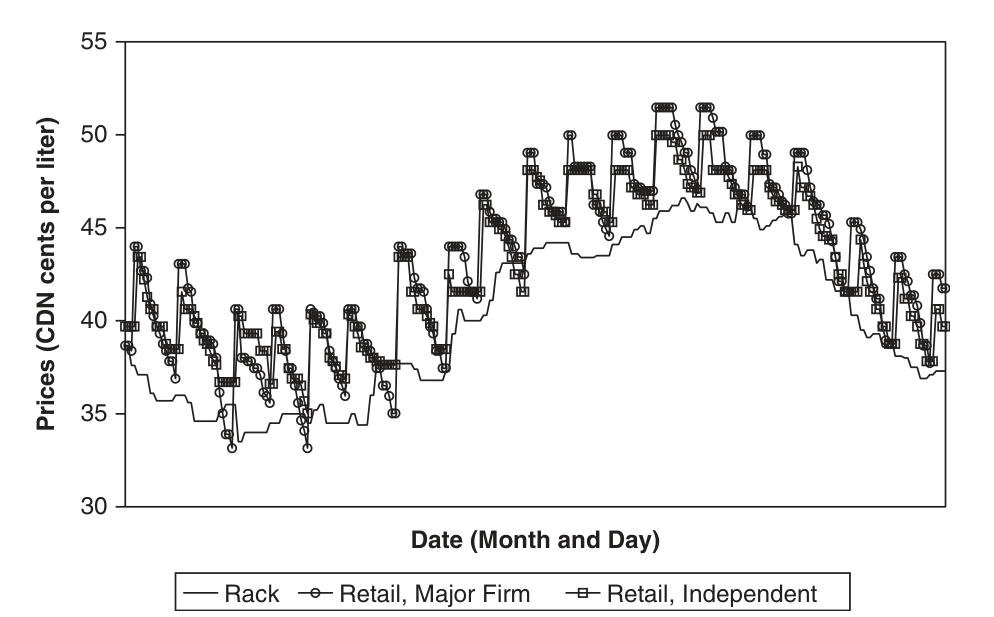
\includegraphics[width=0.78\textwidth]{figures/ch13/noel2007_fig1.png}
\caption{Twelve-hourly retail prices at a major-firm station and an independent station in Toronto, February to
June 2001, with the rack price. Prices exclude taxes. Source: \citet{Noel2007}, Figure 1.}
\label{fig:13-noel-f1}
\end{figure}

\casehead{Model}
For station $s$ in period $t$, the regime $I_{st}\in\{R,U\}$ is either relenting or undercutting. The regime is
latent, because a zero or small change can belong to either phase. Within regime $i$, the price change
$\Delta p_{st}$ follows (Noel's eq.~(4))
\begin{equation}\label{eq:13-noel-regime}
\Delta p_{st}=\begin{cases}X^{i}_{st}\beta^{i}+\epsilon^{i}_{st}, & \text{with probability }1-\gamma^{i}_{st},\\
0, & \text{with probability }\gamma^{i}_{st},\end{cases}\qquad \epsilon^{i}_{st}\sim N(0,\sigma_i^2).
\end{equation}
The mass point at zero allows for stations that skip a period, since the twelve-hour sampling need not match the
true length of a pricing period. The \emph{sticky-price probability} $\gamma^i_{st}$ and the regime transition
probabilities are logits (Noel's eqs.~(5)--(6)):
\begin{equation}\label{eq:13-noel-logits}
\begin{gathered}
\lambda^{iR}_{st}=\Pr\big(I_{st}=R\mid I_{s,t-1}=i,W^i_{st}\big)=\frac{\exp(W^i_{st}\vartheta^i)}{1+\exp(W^i_{st}\vartheta^i)},\qquad
\lambda^{iU}_{st}=1-\lambda^{iR}_{st},\\
\gamma^i_{st}=\frac{\exp(V^i_{st}\zeta^i)}{1+\exp(V^i_{st}\zeta^i)} .
\end{gathered}
\end{equation}
In this subsection $\lambda$ and $\gamma$ are local symbols, and $a_i=\E[\Delta p\mid\Delta p\neq0,\text{regime }i]$
denotes the expected nonzero price change, which Noel writes $\alpha^i$. The density of an observed change in
regime $i$ mixes a point mass and a normal density:
\begin{equation}\label{eq:13-noel-density}
g_i(\Delta p_{st})=\gamma^i_{st}\,\indic\{\Delta p_{st}=0\}+(1-\gamma^i_{st})\,\frac{1}{\sigma_i}\,\phi\Big(\frac{\Delta p_{st}-X^i_{st}\beta^i}{\sigma_i}\Big)\,\indic\{\Delta p_{st}\neq0\},
\end{equation}
where $\phi$ is the standard normal density.
The likelihood is computed with the filter of \cref{sec:13-markov}, following \citet{CosslettLee1985} as in
\citet{Ellison1994}. Let $\xi_{t\mid t-1}(j)$ be the probability of regime $j$ given past price changes. Then
\begin{align*}
\xi_{t\mid t-1}(j)&=\sum_{i\in\{R,U\}}\lambda^{ij}_{st}\,\xi_{t-1\mid t-1}(i),\qquad
f(\Delta p_{st}\mid\text{past})=\sum_{j}\xi_{t\mid t-1}(j)\,g_j(\Delta p_{st}),\\
\xi_{t\mid t}(j)&=\frac{\xi_{t\mid t-1}(j)\,g_j(\Delta p_{st})}{f(\Delta p_{st}\mid\text{past})},\qquad
\ell=\sum_{s}\sum_{t}\ln f(\Delta p_{st}\mid\text{past}).
\end{align*}
The parameters are estimated by maximum likelihood with Newey-West standard errors.

The cycle's characteristics follow from the switching probabilities. With constant probabilities the length of a
spell in regime $i$ is geometric, so its expected duration is $\frac{1}{1-\lambda^{ii}}$ (\cref{lem:13-durations}).
The expected period of the cycle is the sum of the two expected durations. The total price increase during a
relenting spell is the sum of a random number of independent price changes, each with mean $(1-\gamma^R)a_R$.
By Wald's identity its expectation is the product of the mean duration and the mean change:
\begin{equation}\label{eq:13-noel-amplitude}
\E[\text{amplitude}]=\frac{(1-\gamma^R)\,a_R}{1-\lambda^{RR}},\qquad
\E[\text{period}]=\frac{1}{1-\lambda^{RR}}+\frac{1}{1-\lambda^{UU}},\qquad
\text{asymmetry}=\frac{1-\lambda^{RR}}{1-\lambda^{UU}} .
\end{equation}
The asymmetry measure is the ratio of the undercutting duration to the relenting duration. Standard errors come
from the delta method.

\casehead{The anatomy of the cycle}
\Cref{tab:13-noel} reproduces the estimates with constant parameters. The relenting phase lasts 1.008 half-days,
which confirms the structural prediction: each station completes its increase within one twelve-hour period. The
undercutting phase lasts 12.78 half-days, so the cycle repeats about once a week. The amplitude is 5.62 cpl, or 13
percent of the average pre-tax price and 170 percent of the average markup. Increases of 10 cpl in one step were
common in the sample.

\begin{table}[htbp]
\centering
\caption{Regime estimates and cycle characteristics, Toronto 2001}\label{tab:13-noel}
\small
\begin{tabular}{lccc}
\toprule
 & (1) All firms & (2) Major firms & (2) Independents\\
\midrule
\multicolumn{4}{l}{\textit{Relenting phase}}\\
$a_R$ (expected nonzero change, cpl) & 5.576 (0.083) & 5.782 (0.101) & 5.192 (0.142)\\
$\sigma_R$ & 1.650 (0.066) & 1.610 (0.085) & 1.655 (0.100)\\
$\gamma^R$ (sticky share) & 4.0E-5 (4.6E-4) & 4.1E-5 (4.8E-4) & 3.8E-5 (4.9E-4)\\
\multicolumn{4}{l}{\textit{Undercutting phase}}\\
$a_U$ (expected nonzero change, cpl) & $-0.751$ (0.008) & $-0.767$ (0.010) & $-0.720$ (0.015)\\
$\sigma_U$ & 0.459 (0.009) & 0.467 (0.012) & 0.441 (0.012)\\
$\gamma^U$ (sticky share) & 0.429 (0.007) & 0.422 (0.008) & 0.441 (0.014)\\
\multicolumn{4}{l}{\textit{Switching probabilities}}\\
$\lambda^{RR}$ & 0.008 (0.004) & 0.008 (0.005) & 0.007 (0.007)\\
$\lambda^{RU}$ & 0.992 (0.004) & 0.992 (0.005) & 0.993 (0.007)\\
$\lambda^{UR}$ & 0.078 (0.001) & 0.078 (0.002) & 0.078 (0.003)\\
$\lambda^{UU}$ & 0.921 (0.001) & 0.921 (0.002) & 0.921 (0.003)\\
\multicolumn{4}{l}{\textit{Cycle characteristics}}\\
Relenting duration (half-days) & 1.008 (0.004) & 1.008 (0.007) & 1.007 (0.007)\\
Undercutting duration (half-days) & 12.780 (0.291) & 12.779 (0.358) & 12.784 (0.484)\\
Cycle period (half-days) & 13.788 (0.291) & 13.787 (0.358) & 13.792 (0.485)\\
Asymmetry & 12.680 (0.291) & 12.677 (0.363) & 12.687 (0.491)\\
Amplitude (cpl) & 5.619 (0.082) & 5.828 (0.098) & 5.232 (0.144)\\
\bottomrule
\end{tabular}

\smallskip
\begin{minipage}{0.92\textwidth}\footnotesize
Notes: Specification (1) has no firm-type dummies. Specification (2) adds major and independent dummies to $a_i$,
$\lambda^{ij}$ and $\gamma^i$. Standard errors from the delta method in parentheses. Source: \citet{Noel2007},
Tables II and III.
\end{minipage}
\end{table}

\begin{example}[Checking the cycle arithmetic]\label{ex:13-noel-cycle}
From \eqref{eq:13-noel-amplitude}, the relenting duration is $\frac{1}{1-0.008}=1.008$. The undercutting duration of
12.780 implies an unrounded $\lambda^{UU}=1-\frac{1}{12.780}=0.9218$. This rounds to 0.922, one unit in the third
decimal above the 0.921 that the table reports. The period is
$1.008+12.780=13.788$ half-days and the asymmetry is $\frac{12.780}{1.008}=12.68$. The amplitude is
$(1-0.00004)\times5.576\times1.008=5.62$ cpl, equal to the reported 5.619 up to rounding. The descent can be checked
the same way. The expected change per half-day in the undercutting phase is $(1-0.429)\times(-0.751)=-0.43$ cpl, and
over 12.78 half-days prices fall by $0.43\times12.78=5.48$ cpl. Up and down movements nearly balance over a cycle, as
they must when prices show no strong trend over the sample.
\end{example}

\casehead{Small versus large firms}
To test the behavioral predictions, Noel lets the parameters depend on two variables, interacted with firm type.
The first, $\textit{POSITION}_{st}=\textit{RETAIL}_{s,t-1}-\textit{RACK}_{st}-\textit{TAX}_{st}$, measures how far the
station's pre-tax price is above the bottom of the cycle. The second, $\textit{FOLLOW}_{st}$, equals one if some other
station has already relented and station $s$ has not. The probability of switching from undercutting to relenting
rises steeply as margins shrink. For majors it is 0.046 at the mean \textit{POSITION} of 3.31 cpl and 0.110 at 1.53,
the mean just before a relent. It reaches 0.272 at zero and 0.803 at the minimum of $-3.24$ (Table IV). At
$\textit{POSITION}=1.53$ the derivative $\frac{\partial\lambda^{UR}}{\partial\,\textit{POSITION}}$ is $-0.065$ (0.006)
for majors and $-0.051$ (0.006) for independents.

Prediction (2) holds. Near the top of the cycle independents undercut more often and majors keep sticky prices.
Near the bottom the roles reverse. The derivative of the sticky-price probability with respect to \textit{POSITION} is
0.036 (0.002) for majors and $-0.034$ (0.005) for independents (Table V). Large firms try to hold high prices for a
while, then chase the small firms down. Just before a relent majors are often cheaper than independents.

Prediction (3) holds as well, and \cref{tab:13-noel-t5} shows it. When no station has yet relented, a major
relents in a given half-day with probability 0.091 and an independent with probability 0.026. Once some station has
relented, a major follows within half a day with probability 0.925 and an independent with probability 0.720. Both
probabilities are high, which confirms prediction (1): reactions are fast but not simultaneous. With data sampled
every two days or less often, the increases would look perfectly synchronous. A major that follows raises its price
by 0.200 cents less than if it had led, which is the predicted undercut of the leader by the follower. The relenting
jump falls almost one for one with \textit{POSITION} (derivatives $-0.897$ for majors and $-0.873$ for independents),
so stations restore a nearly standard markup.

\begin{table}[htbp]
\centering
\caption{Leaders and followers: probability of switching from undercutting to relenting in a half-day}\label{tab:13-noel-t5}
\small
\begin{tabular}{lcccc}
\toprule
 & \multicolumn{2}{c}{Leaders (no station has relented)} & \multicolumn{2}{c}{Followers (some station has relented)}\\
\cmidrule(lr){2-3}\cmidrule(lr){4-5}
 & Majors & Independents & Majors & Independents\\
\midrule
$\textit{POSITION}=1.53$ & 0.091 (0.006) & 0.026 (0.003) & 0.925 (0.045) & 0.720 (0.045)\\
$\textit{POSITION}=0$ & 0.235 (0.020) & 0.066 (0.011) & 0.974 (0.016) & 0.868 (0.030)\\
\bottomrule
\end{tabular}

\smallskip
\begin{minipage}{0.92\textwidth}\footnotesize
Notes: Entries are $\lambda^{UR}$ from specification (4), in which the relenting jump and the switching probability
depend on firm type, \textit{FOLLOW}, \textit{POSITION} and their interactions. Delta-method standard errors in
parentheses. A \textit{POSITION} of 1.53 cpl is the average just before a relent. Source: \citet{Noel2007}, Table V.
\end{minipage}
\end{table}

\casehead{Competing hypotheses}
Noel rejects four alternatives to Edgeworth cycles. A day-of-the-week demand cycle cannot produce one large jump
followed by daily declines. The jump falls on different weekdays, and periods range from four to ten days. Relents
do cluster early in the week. The first relent of a round comes on Monday 18 percent of the time, Tuesday 32,
Wednesday 22, Thursday 18, Friday 10 and never at weekends. Differences in menu or monitoring costs cannot explain why majors move
faster upward but not downward. Inventory depletion would require station managers to misforecast their sales in the
same direction every period, and deliveries occur on different days for different stations. Rack-price discounts are
below 1 cpl, against an amplitude of 5.6 cpl, and do not vary over time.

The fifth alternative, covert collusion, cannot be excluded by any price pattern, since the folk theorem
(\cref{ch:collusion-theory}) admits many collusive paths. Noel argues that a cycle is an implausible collusive scheme.
Simple rules such as a constant markup are easier to agree on and to monitor. Cycles require fast, differentiated price
moves at hundreds of stations, and their large jumps attract complaints. The data also show no single price leader:
different firms lead the relents, and the ranking of stations changes often during the descent.

\casehead{Interpretation and critiques}
The evidence supports a competitive reading of the Toronto cycle. Its price wars are not punishments: prices fall
repeatedly and predictably as firms compete, and informed consumers can lower what they pay by timing purchases. An
informal poll of 58 residents found that they expected 58 percent of price changes to be increases, whereas 86 percent
of actual changes were decreases. The study has clear limits. It has no quantity data, so it cannot measure welfare or
the station-level elasticity behind the fast undercutting. The sample is 22 stations over 131 days. The tests are
consistency tests, since the theory leaves the amplitude and the top price undetermined. The main caveat for
detection comes from Quebec. \Cref{sec:13-clarkhoude} shows that a documented cartel there also produced asymmetric
cycles. The shape
of the cycle cannot by itself separate competition from collusion. The role assignments of small and large firms carry
more of the evidential weight than the shape. Later work exploits sharper variation, for example a regulation of the
timing of price changes in Perth studied by \citet{Wang2009}.

\subsection{A prosecuted cartel with asymmetric retailers: Clark and Houde (2013)}\label{sec:13-clarkhoude}

\casehead{Question}
Repeated-game theory has long recognized that firms with different costs or sizes need side payments to collude
\citep{JacqueminSlade1989}. Upstream cartels can assign quotas or territories. In a retail market with posted prices,
however, a cartel cannot tell consumers where to shop. At a common price, market shares follow locations and
amenities. They need not match what each firm requires to stay in the cartel. \citet{ClarkHoude2013} ask how a cartel of heterogeneous gasoline
retailers solved this problem, using the record of a prosecuted case.

\casehead{Setting and data}
The cartel came to light after a Victoriaville newspaper published, on June 6, 2004, an interview with station owner
Christian Goulet. He claimed he was harassed for refusing to go along with price fixing. The Canadian Competition
Bureau began recording phone conversations on March 3, 2005 and executed search warrants from May 29, 2006. Charges were
announced on June 12, 2008, with later rounds in 2010 and 2012, against fourteen companies and thirty-nine individuals
in total. By September 2012 seven companies and 27 individuals had pleaded guilty, with company fines from \$90,000 to
\$1,850,000. The case covers 128 stations and 64 firms in Victoriaville, Thetford Mines, Sherbrooke and Magog.

Three sources are combined. The Competition Bureau's court documents summarize or quote the recorded calls for each price
change, with caller, receiver and time. A weekly station-level survey by the Quebec energy board (the R\'egie de
l'\'energie) covers 2002--2005. A quarterly survey by Kent Marketing reports volumes, characteristics and the full
cross-section of prices. The key players differ sharply. Bilodeau (Shell) organized the cartel in Victoriaville and
Thetford Mines and Bourassa (Olco) in Sherbrooke. Both run the largest networks of lessee stations. Ultramar, the only
refiner in eastern Quebec, sets prices centrally and runs a low-price guarantee that commits its stations to post the
lowest price in each neighborhood. Two big-box retailers, Canadian Tire and Maxi, run high-volume stations as loss leaders.
Couche-Tard, the largest convenience-store chain, sets prices through one regional representative.

\casehead{Heterogeneous costs}
Station sizes vary widely. The average Sherbrooke station sells 48.67 thousand liters a week with a standard deviation
of 24.56 (Table 2). Following \citet{Houde2012}, marginal cost is additive in the \emph{minimum estimated price} (MEP), a
weekly price floor published by the R\'egie that stations may not undercut:
\begin{equation}\label{eq:13-ch-mc}
mc_{jt}=\textit{MEP}_t+c_j .
\end{equation}
The station cost differential $c_j$ comes from \citet{Houde2012}. He recovers station marginal costs by inverting the
multi-product Bertrand first-order conditions of a spatial demand model (\cref{ch:diffprod}) and regresses them on station
characteristics. Stations with more pumps, a convenience store or a car wash have lower costs. The differentials range
from $-0.05$ to $-1.98$ cpl in Sherbrooke and from $-0.02$ to $-2.03$ cpl in Victoriaville. Ultramar's stations are on
average 1.6 cpl below the MEP.

\casehead{Price patterns}
Weekly price changes in the cartel cities from 2002 to 2005 form an asymmetric cycle (\cref{fig:13-ch-f1}). Increases are
spread symmetrically around 4 cpl, with an interquartile range of 2 cpl. Cuts cluster at 1 or 2 cpl, and 70 percent are at
most 2 cpl. Floor changes are much more symmetric, so prices rise faster than they fall. Prices were unchanged two weeks in a
row 48 percent of the time in Victoriaville, 57 percent in Thetford Mines and 36 percent in Sherbrooke. The floor was
constant only 1.2 percent of the time. In Victoriaville and Thetford Mines, 95 percent of price changes kept the ending digit
fixed. The cross-section of prices was
concentrated. In Victoriaville the suggested price was 2 cpl above the minimum, and two fringe stations were allowed to post
up to 2 cpl below it. In Thetford Mines self-service stations posted half a cent below full-service ones.

\begin{figure}[htbp]
\centering
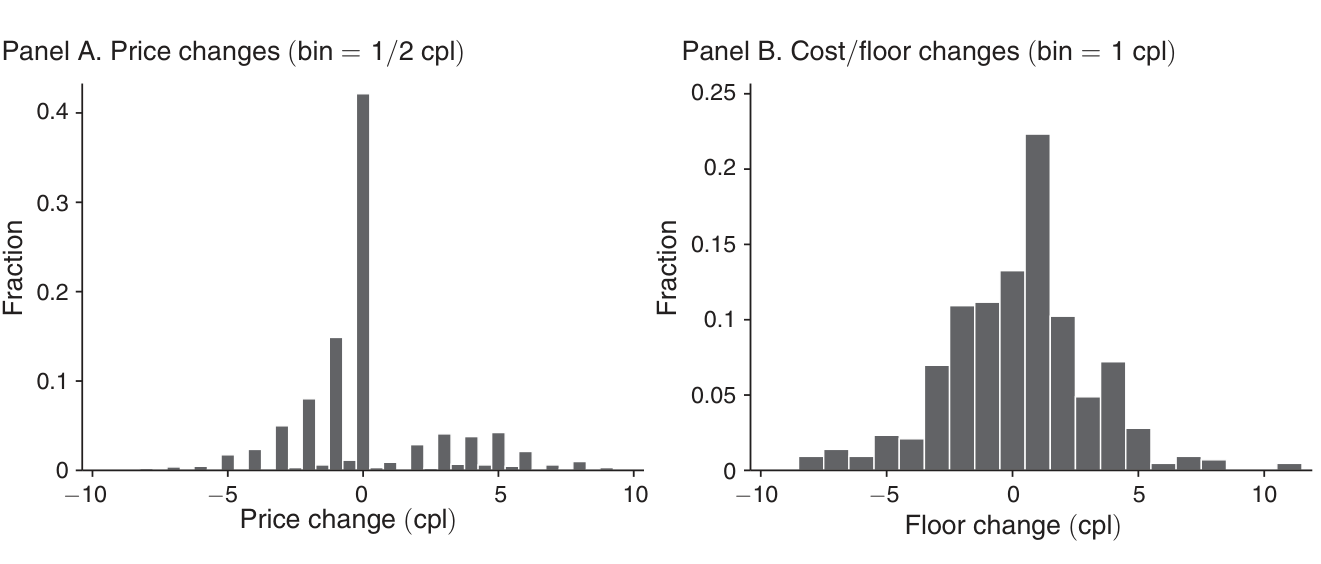
\includegraphics[width=0.88\textwidth]{figures/ch13/clarkhoude2013_fig1.png}
\caption{Distribution of weekly price changes (panel A) and of price-floor changes (panel B) in the cartel cities,
2002--2005. Source: \citet{ClarkHoude2013}, Figure 1.}
\label{fig:13-ch-f1}
\end{figure}

\casehead{Why asymmetry is a problem: a two-firm model}
The authors illustrate the enforcement problem with two retailers of a homogeneous good facing inelastic unit demand.
Firm $H$ has marginal cost $c>0$ and firm $L$ has cost 0. At the cartel price $\bar p$ they hold shares $s_H$ and
$s_L=1-s_H$. After a deviation they play static Bertrand forever, in which $H$ earns zero and $L$ serves the market at price
$c$. The incentive constraints are
\begin{equation}\label{eq:13-ch-ic2}
\textit{IC}^H:\ \frac{s_H(\bar p-c)}{1-\delta}\ge p^d_H-c,\qquad
\textit{IC}^L:\ \frac{s_L\bar p}{1-\delta}\ge p^d_L+\delta\,\frac{c}{1-\delta},
\end{equation}
where $p^d_j$ is the deviation price. The low-cost firm loses less from the punishment, because it keeps the whole market
at price $c$.

\begin{proposition}[Collusion needs an unequal split]\label{prop:13-ch-shares}
In the two-firm model, let deviations undercut $\bar p$ by an arbitrarily small amount. Collusion at $\bar p$ is sustainable
if and only if
\begin{equation*}
\delta\ge\underline\delta(s_L)\equiv\max\Big\{s_L,\ \frac{(1-s_L)\,\bar p}{\bar p-c}\Big\}.
\end{equation*}
The threshold is minimized at $s_L^*=\frac{\bar p}{2\bar p-c}>\frac{1}{2}$, where $\underline\delta(s_L^*)=\frac{\bar p}{2\bar p-c}$.
With equal shares the threshold is $\frac{\bar p}{2(\bar p-c)}$, which is at least one when $c\ge\frac{\bar p}{2}$,
so collusion with equal shares is then impossible for every $\delta<1$.
\end{proposition}

\begin{proof}
Let $p^d_H,p^d_L\to\bar p$. Multiplying $\textit{IC}^H$ by $1-\delta$ gives $s_H(\bar p-c)\ge(1-\delta)(\bar p-c)$, or
$\delta\ge1-s_H=s_L$. Multiplying $\textit{IC}^L$ by $1-\delta$ gives
\begin{equation*}
s_L\bar p\ge(1-\delta)\bar p+\delta c,
\end{equation*}
which rearranges to $\delta(\bar p-c)\ge(1-s_L)\bar p$, or $\delta\ge\frac{(1-s_L)\bar p}{\bar p-c}$. Both must hold, which gives
the maximum. The first term increases in $s_L$ and the second decreases, so the maximum is smallest where they are equal:
$s_L(\bar p-c)=(1-s_L)\bar p$, or $s_L^*=\frac{\bar p}{2\bar p-c}$. Since $c>0$, $s_L^*>\frac{1}{2}$. Substituting $s_L=\frac{1}{2}$
gives $\max\{\frac{1}{2},\frac{\bar p}{2(\bar p-c)}\}=\frac{\bar p}{2(\bar p-c)}$, which is at least one when $\bar p\le2c$.
\end{proof}

The proposition is our formalization of the authors' example. With a large cost gap, collusion on equal shares is
impossible at any discount factor, while a split that favors the low-cost firm sustains it for $\delta$ close to one. The
cartel thus faces an \emph{enforcement problem}, which requires shifting market share toward low-cost and small-network
firms. It also faces a \emph{coordination problem}, because firms with different deviation gains disagree about the price.
In posted-price retail the cartel cannot set $s_L$ directly. It has to create temporary price differences that move volume
toward the firms it needs to keep on board.

\casehead{The mechanism: a coordinated order of play}
The court documents show how. A price increase works like a negotiation. The leader first agrees with Couche-Tard and the
active followers on a target price and a time $t_0$ at which most stations raise their prices. The leader then contacts
Ultramar and the big-box retailers and proposes a later time $t_1\ge t_0$ for their increase. Dissident stations, which are
independents with large capacity or outlying locations, are told of the increase directly or indirectly. A typical
Victoriaville increase involved about 65 calls, many between the leader and Couche-Tard (Table 3). Low-cost stations and
dissidents received far more calls than they made. The delay was explicit. When a station owner said he would wait for the
neighboring Ultramar station, Bilodeau replied: ``I know that, I'm not worried, it's always the same thing.'' An Ultramar
manager described the arrangement in these words. ``We built the system seven years ago, the competitors know that the program
belongs to us and we want to be sure that we are the last one to move [up].''

Most stations raise their prices at once, while a group delays by up to four hours in Victoriaville and 80 minutes in Thetford
Mines (Figure 3). \Cref{tab:13-ch-t4} regresses each station's delay on station categories and episode characteristics.
Relative to the leader's stations, Ultramar and the big-box stations raise their prices about two and a half hours later in
Victoriaville and about an hour later in Thetford Mines. Larger proposed increases shorten the delays. A larger increase makes
the delay more costly for early movers and more valuable for late movers, so the cartel grants less time. Delays are longer when
more than 20 days have passed since the last increase, because the transfer then accumulates over a longer interval. Price
decreases are different. Ultramar initiates them without warning, nine of the ten documented decreases in Victoriaville and three
of the four in Thetford Mines. Others match quickly without retaliation, and a decrease involves about 26 calls. The low-price
guarantee makes Ultramar the natural leader of cuts and saves the cartel the cost of coordinating them. The leader's role on
the way down is to warn followers quickly, so that they stay competitive and do not cut on their own. A linear probability
model of who receives such a warning (Table 6 of the paper) shows that the low-cost chains are rarely called, because they
start the cuts. In the pooled sample, followers are 25 percent less likely to be warned than the leader's own stations.

\begin{table}[htbp]
\centering
\caption{Price-increase delays (minutes after the leader's stations) and station characteristics}\label{tab:13-ch-t4}
\small
\begin{tabular}{lcc}
\toprule
 & (1) Victoriaville & (2) Thetford Mines\\
\midrule
Dissident stations & 157.6$^{***}$ (37.88) & \\
Low-cost chains (Ultramar, big-box) & 149.4$^{***}$ (21.33) & 64.70$^{***}$ (9.206)\\
Follower stations & 37.41$^{**}$ (15.75) & 13.71$^{*}$ (7.019)\\
Couche-Tard stations & 23.68 (23.50) & $-13.74^{***}$ (4.879)\\
Distance to low-cost chains & 8.676 (10.18) & $-2.074^{***}$ (0.773)\\
Distance to closest competitor & $-14.51$ (15.09) & $-6.920^{***}$ (2.439)\\
Proposed increase & $-35.06^{***}$ (4.794) & $-11.35^{*}$ (6.135)\\
Current margin & $-40.50^{***}$ (2.977) & $-6.582^{**}$ (2.563)\\
Last increase $\ge20$ days ago & 76.21$^{***}$ (17.59) & 19.60 (19.53)\\
Constant & 215.3 (136.4) & 161.1$^{***}$ (48.17)\\
\addlinespace
Observations & 122 & 83\\
$R^2$ & 0.657 & 0.535\\
\bottomrule
\end{tabular}

\smallskip
\begin{minipage}{0.86\textwidth}\footnotesize
Notes: OLS, robust standard errors in parentheses. The reference group is the leader's network. Delays of dissidents are observed
only when they cooperated, and the actions of the two Thetford Mines dissidents are never observed. $^{***}$, $^{**}$, $^{*}$:
significant at 1, 5, 10 percent. Source: \citet{ClarkHoude2013}, Table 4 (the regression of delays).
\end{minipage}
\end{table}

\casehead{The value of delay: demand model}
To measure the transfer, the authors model a firm that may raise its price late, or cut it early. It receives a fraction
$\tau_t$ of the week's demand at the initial price vector. The paper writes $\alpha_t$ for this share and $\gamma$ for the price
coefficient. We use $\tau_t$ and $\alpha$ to keep the book's notation, in which $\alpha$ is the price coefficient. The documents suggest delays of about half a day on increases and thirty minutes on decreases, at most once a
week. With uniform demand over twelve open hours a day, this would be $\frac{1}{14}$ and $\frac{1}{168}$ of weekly sales.
Predictable increases and the price dispersion they create make consumers time their purchases, so the authors set
$\tau=\frac{1}{7}$ for increases and $\tau=\frac{1}{140}$ for decreases. Three firms (Ultramar, Maxi and Canadian Tire) may delay
increases and only Ultramar may lead cuts.

Two demand models bracket the truth. In the homogeneous model consumers buy at the cheapest station, shares are $\frac{1}{N}$ at
equal prices, and low-price stations serve the whole market during a delay. The market size is the population of Victoriaville
times three liters a day. The logit model (\cref{ch:logit}) gives station $j$ the demand
\begin{equation}\label{eq:13-ch-logit}
D_j(\mathbf p_t)=M\,\frac{\exp(X_{jt}\beta+\xi_{q}-\alpha p_{jt})}{\exp(-\alpha p_{0t})+\sum_k\exp(X_{kt}\beta+\xi_{q}-\alpha p_{kt})}.
\end{equation}
Mean quality $X_{jt}\beta+\xi_q$ depends on size and amenities $X_{jt}$ and on a quarter effect $\xi_q$. The paper writes it as
$\delta_{jt}$, a symbol that this chapter reserves for the discount factor. The price $p_{0t}$ is the average price in neighboring
markets, and $M$ is market size. Let $\tilde{\mathbf p}_t$ be the price vector at the start of the week, before
late movers adjust, and let $\mathcal T_t$ be the set of firms receiving a transfer. Demand with delays is
\begin{equation}\label{eq:13-ch-delay}
D_{j,t}(\mathbf p_t,\tau_t)=\begin{cases}\tau_tD_j(p_{j,t-1},\tilde{\mathbf p}_{-j,t})+(1-\tau_t)D_j(\mathbf p_t), & j\in\mathcal T_t,\\
\tau_tD_j(p_{j,t},\tilde{\mathbf p}_{-j,t})+(1-\tau_t)D_j(\mathbf p_t), & j\notin\mathcal T_t.\end{cases}
\end{equation}
During an increase a receiver keeps its old, lower price for the fraction $\tau_t$ of the week while the others have already
moved. The demand parameters $\Theta^{\mathrm d}=(\alpha,\beta,\xi)$ are estimated by nonlinear least squares on quarterly Kent
volumes $\hat Q_{jq}$ for Victoriaville, 2001--2007:
\begin{equation}\label{eq:13-ch-nls}
\min_{\Theta^{\mathrm d}}\sum_j\sum_q\Big(\log\hat Q_{jq}-\log Q_{jq}(\Theta^{\mathrm d})\Big)^2,\qquad
Q_{jq}(\Theta^{\mathrm d})=\sum_{t\in q}D_{j,t}(\mathbf p_t,\tau_t\mid\Theta^{\mathrm d}).
\end{equation}
The estimated coefficient on price in utility is $-0.409$, with prices in cents per liter, so $\hat\alpha=0.409$. It implies a
store-level elasticity of about $-30$. In the logit model the own elasticity is $-\alpha p_j(1-s_j)$, and shares are only
0.01--0.03 (Table 2). An elasticity of $-30$ therefore corresponds to $p_j(1-s_j)\approx\frac{30}{0.409}=73$ cents per liter
(our computation). Identification comes mostly from the two
dissident stations that priced 2 cpl below the cartel price and from the collapse of price dispersion after the cartel ended. One
of these stations lost half of its market share after the collapse. Prices are treated as exogenous given quarter effects and
characteristics. The authors note that the dissidents were not randomly assigned, so $\hat\alpha$ may be biased.
\citet{Houde2012} obtains a lower average elasticity of $-15$ with bimonthly Quebec data.

\casehead{Results: volume transfers}
\Cref{tab:13-ch-t7} reports the simulated change in each group's sales when the delays are switched on. Increases occur in only
16--23 percent of weeks but are large, so they generate sizable transfers. The low-cost firms gain about 4 percent of volume in
Victoriaville and about 6 percent in Sherbrooke and Thetford Mines. The two demand models give similar answers except in
Victoriaville. There the homogeneous model ignores the unequal shares created by location and amenities and predicts larger gains.

\begin{table}[htbp]
\centering
\caption{Simulated change in sales volume from the delay scheme}\label{tab:13-ch-t7}
\small
\begin{tabular}{llcccccc}
\toprule
 & & \multicolumn{2}{c}{Share of weeks with} & \multicolumn{2}{c}{Logit demand} & \multicolumn{2}{c}{Homogeneous demand}\\
\cmidrule(lr){3-4}\cmidrule(lr){5-6}\cmidrule(lr){7-8}
Market & Players & increase & decrease & Percent & 1,000 l. & Percent & 1,000 l.\\
\midrule
Sherbrooke & Ultramar & 0.225 & 0.373 & 0.061 & 6,759.584 & 0.055 & 733.012\\
 & Big-box & 0.224 & 0.372 & 0.059 & 773.265 & 0.047 & 651.790\\
 & Other & 0.223 & 0.370 & $-0.014$ & $-275.124$ & $-0.035$ & $-442.205$\\
Thetford Mines & Ultramar & 0.169 & 0.350 & 0.064 & 895.420 & 0.056 & 763.006\\
 & Other & 0.168 & 0.349 & $-0.009$ & $-52.570$ & $-0.027$ & $-337.746$\\
Victoriaville & Ultramar & 0.164 & 0.284 & 0.040 & 522.315 & 0.079 & 752.152\\
 & Big-box & 0.164 & 0.284 & 0.038 & 366.553 & 0.054 & 515.890\\
 & Other & 0.161 & 0.288 & $-0.010$ & $-79.329$ & $-0.025$ & $-215.419$\\
\bottomrule
\end{tabular}

\smallskip
\begin{minipage}{0.92\textwidth}\footnotesize
Notes: ``Percent'' entries are proportional changes (0.061 is 6.1 percent) in total sales volume over the collusive period when
the delay scheme is added to the simulation. The entry 6,759.584 is reproduced as printed, although it is about ten times
the neighboring entries. Source: \citet{ClarkHoude2013}, Table 7.
\end{minipage}
\end{table}

\casehead{Results: delays and cartel stability}
To study stability, the authors take the observed price path from January 2002 to October 2004 as the collusive path, with one
common price $p_t$ per week. Information is perfect, so price wars occur only off the path. Punishment sets prices at a floor for
$T$ weeks, either the MEP or the ``long-run'' floor of MEP plus 3 cpl, after which collusion resumes. The big-box stations receive
an extra 2 cpl cost advantage to capture their loss-leader motive, which puts their differential near $-3$ cpl against Ultramar's
$-2.03$. Firm $f$, owning stations $\mathcal J_f$, earns in week $t$
\begin{equation*}
\Pi_{f,t}=\begin{cases}\sum_{j\in\mathcal J_f}\big[\tau_t\pi_j(p_{j,t-1},\tilde{\mathbf p}_{-j,t})+(1-\tau_t)\pi_j(\mathbf p_t)\big], & f\in\mathcal T_t,\\
\sum_{j\in\mathcal J_f}\big[\tau_t\pi_j(p_{j,t},\tilde{\mathbf p}_{-j,t})+(1-\tau_t)\pi_j(\mathbf p_t)\big], & f\notin\mathcal T_t,\end{cases}
\qquad \pi_j(\mathbf p)=D_j(\mathbf p)\,(p_j-mc_{jt}).
\end{equation*}
An agreement $\mathcal A=\{p_t,\tau_t,\mathcal T_t,T\}_{t\ge0}$ is enforceable if every firm prefers cooperation at every date:
\begin{equation}\label{eq:13-ch-ic}
V^{c}_{f,t}(\mathcal A)-V^{d}_{f,t}(\mathcal A)=\sum_{s=0}^{T}\delta^{s}\,\Pi_{f,t+s}-\Big[\Pi^{d}_{f,t}+\sum_{s=1}^{T}\delta^{s}\,\Pi^{p}_{f,t+s}\Big]\ge0 .
\end{equation}
Collusion resumes after the punishment, so the cooperation and deviation paths coincide from $t+T+1$ on and the comparison stops
at $T$. The deviation profit $\Pi^d_{f,t}$ is the best one-week profit from undercutting all of the firm's stations by a whole
number of cents, and $\Pi^p_{f,t}=\sum_{j\in\mathcal J_f}\pi_j(\mathbf p^f_t)$ is profit at the floor. The weekly discount factor is
0.99. The deviation frequency is the share of firm-weeks at which \eqref{eq:13-ch-ic} fails. The minimum punishment $T^*$ is the
shortest war that prevents every deviation in the sample.

\Cref{tab:13-ch-t8} shows that delays matter at intermediate punishment lengths. With very short or very long wars the
deviation frequency is one or zero with or without transfers. In between, the delays lower it. They also shorten the war needed
to deter all deviations. In the homogeneous model the saving is 27 weeks with the high floor and 9 weeks with the low floor. In the
logit model it is 6 weeks with the high floor and zero with the low floor. A higher floor weakens punishments, and less
differentiation raises the gain from undercutting. In both cases the cartel is less stable, and transfers become more valuable.

\begin{table}[htbp]
\centering
\caption{Deviation frequencies and minimum punishment lengths, Victoriaville}\label{tab:13-ch-t8}
\small
\begin{tabular}{llcccccc}
\toprule
\multicolumn{2}{c}{Specification} & \multicolumn{4}{c}{Deviation frequency} & \multicolumn{2}{c}{Minimum punishment $T^*$}\\
\cmidrule(lr){1-2}\cmidrule(lr){3-6}\cmidrule(lr){7-8}
Floor & Demand & $T=4$ & $T=8$ & $T=32$ & $T=52$ & Delays & No delays\\
\midrule
$\textit{MEP}_t+3$ & logit & \makecell{0.868\\(0.017)} & \makecell{0.516\\(0.085)} & 0.009 & 0.000 & 35 & 41\\
\addlinespace
$\textit{MEP}_t$ & logit & \makecell{0.460\\(0.073)} & \makecell{0.078\\(0.004)} & 0.000 & 0.000 & 15 & 15\\
\addlinespace
$\textit{MEP}_t+3$ & homogeneous & \makecell{1.000\\(0.000)} & \makecell{0.981\\(0.016)} & \makecell{0.636\\(0.104)} & \makecell{0.394\\(0.406)} & 144 & 171\\
\addlinespace
$\textit{MEP}_t$ & homogeneous & \makecell{1.000\\(0.000)} & \makecell{0.956\\(0.022)} & \makecell{0.340\\(0.435)} & \makecell{0.071\\(0.286)} & 67 & 76\\
\bottomrule
\end{tabular}

\smallskip
\begin{minipage}{0.92\textwidth}\footnotesize
Notes: Share of firm-weeks, January 2002 to November 2004, in which the incentive constraint \eqref{eq:13-ch-ic} fails, with the
delay transfers. Numbers in parentheses are the proportional change in that frequency when the transfers are removed. $T^*$ is the
shortest punishment, in weeks, with no deviation in the sample. Source: \citet{ClarkHoude2013}, Table 8.
\end{minipage}
\end{table}

\Cref{tab:13-ch-t9} measures who gains. With logit demand the delays raise the net value of collusion for the three receivers by
3 to 13 percent. With homogeneous demand the gains range from 17 to 53 percent. The early movers, 88 percent of firms, lose
between 1 and 5 percent on average.
Ultramar gains least, because its two-station network already gains less from deviating. Network size, more than cost, emerges
as the main source of asymmetry, partly because the floor limits the effect of cost differences.

\begin{table}[htbp]
\centering
\caption{Net value of the delay transfers, Victoriaville (thousands of dollars)}\label{tab:13-ch-t9}
\small
\begin{tabular}{llcccc}
\toprule
Floor & Demand & Canadian Tire & Maxi & Ultramar & Others\\
\midrule
$\textit{MEP}_t+3$ & logit & 14.956 (0.129) & 17.000 (0.127) & 7.373 (0.075) & $-1.685$ ($-0.025$)\\
$\textit{MEP}_t$ & logit & 15.424 (0.049) & 17.471 (0.048) & 7.478 (0.032) & $-1.577$ ($-0.011$)\\
$\textit{MEP}_t+3$ & homogeneous & 41.892 (0.523) & 42.195 (0.531) & 46.386 (0.273) & $-4.528$ ($-0.051$)\\
$\textit{MEP}_t$ & homogeneous & 44.420 (0.290) & 44.736 (0.294) & 47.985 (0.168) & $-5.695$ ($-0.032$)\\
\bottomrule
\end{tabular}

\smallskip
\begin{minipage}{0.92\textwidth}\footnotesize
Notes: Change in the net value of cooperation $V^c_{f,t}-V^d_{f,t}$ when the delays are added, evaluated at the minimum
punishment $T^*$ without delays (last column of \cref{tab:13-ch-t8}). Proportional changes in parentheses. ``Others'' is the
average over the firms that move early. Source: \citet{ClarkHoude2013}, Table 9.
\end{minipage}
\end{table}

\casehead{Interpretation}
The Quebec cartel solved its enforcement problem with intertemporal transfers implemented through the order of play. The
transfers resemble the sales-based payments of \citet{HarringtonSkrzypacz2011} (\cref{ch:collusion-theory}) and the sidepayments
of Asker's bidding ring (\cref{sec:13-asker}). Their currency is time, and the timing is predictable and agreed in advance. \Citet[p.~122]{ClarkHoude2013}
compare the pricing rule of large, infrequent increases followed by small cuts or constant prices to an $(s,S)$ rule. The term comes from inventory theory. An $(s,S)$ rule leaves a state variable alone until it falls to a lower trigger
$s$ and then resets it to a higher target $S$. Here the state is the margin, which drifts down through small cuts until the
cartel restores it with one large coordinated increase. The analogy concerns only this pattern of rare, discrete resets. The
paper does not study the optimal timing or size of price changes (p.~121), and it estimates no thresholds $s$ and $S$. The
rule economizes on the costly and risky communication needed to coordinate increases, while a constant-markup rule would
require frequent coordinated changes as costs move. The two signatures that antitrust authorities usually look for, parallel price changes and stable
margins, are both absent. Sequential moves and asymmetric cycles can be part of a collusive agreement.
\citet[p.~121]{ClarkHoude2013} report that their companion paper \citep{ClarkHoude2014} finds a substantial fall in price
asymmetry in all four cities after the search warrants were executed. The fall stems largely from larger price cuts, once the cartel
could no longer prevent firms from undercutting their rivals.

\casehead{Critiques}
The analysis relies on summaries of conversations selected by investigators. Only a few price increases are common to all
stations, so the standard errors of the episode variables are understated, as the authors note. The price coefficient comes from
non-random variation. The stability exercise assumes perfect information and immediate punishment, whereas the two documented
deviations were met with weeks of threats and negotiation before a price war began. The model treats the delay as given. A full
account would let firms bargain over delays and prices \citep{Harrington1991}. The price floor regulation is specific to Quebec, and it
shapes both the cost function and the punishment.

\casehead{Contribution}
The paper is among the first to document the internal organization of a retail cartel. It identifies a transfer mechanism suited to
posted-price markets, quantifies it with demand models, and shows through a structural incentive-constraint exercise when it matters
for stability. Its main message for detection is that collusion and competitive Edgeworth cycles can generate similar price paths.

\subsection{The end of the cartel as a natural experiment: Erutku and Hildebrand (2010)}\label{sec:13-erutku}

\casehead{Question and setting}
When an investigation becomes public, a cartel may collapse. \citet{ErutkuHildebrand2010} use the public announcement of the Quebec
investigation to estimate the overcharge in Sherbrooke, the largest of the four cities. Sherbrooke has close to 150,000 residents and
about 60 stations (Table 1). Court documents report 16 price increases or attempted increases between April 1, 2005 and April 18, 2006.
The Bureau's documents give different counts of the participants (p.~224, note~2). The number of conspirators in Sherbrooke is 53, 54
or 63, and the number of stations 64, 65 or 66. With 53 participants and 66 stations, at least 80 percent of the stations took part at
some point. On May 29, 2006 the Bureau's officers raided stations in the Sherbrooke-Victoriaville area, and on June 2 the Commissioner
of Competition publicly confirmed the investigation. The authors treat these events together as the announcement. On June 12, 2008
the Commissioner announced criminal charges against 13 individuals and 11 companies in the four cities. Fines on the parties that
pleaded guilty totaled over \$2 million, and the Bureau's immunity program offered protection to the first party to disclose the
offense (p.~224).

The market structure is unusual for a prosecuted cartel. In the price-fixing cases brought by the U.S.\ Department of Justice from
1963 to 1972, 49 of 62 cases had ten or fewer conspirators. The four-firm concentration ratio exceeded 50 percent in 38 of the 50 cases
with data (our tabulation of Hay and Kelley's table as reproduced in \citealp[Table~2]{ErutkuHildebrand2010}). In Sherbrooke at least
50 different individuals coordinated price increases (p.~227). The market was not concentrated, with a Herfindahl index below 1,800.
Ultramar, the largest retailer with 14 outlets, came close to being a maverick. Its Value Plus program promised prices no higher than
competitors' lowest prices in each price zone, so Ultramar followed an increase only after every other station had raised its price.
Sometimes it waited so long that the agreed increase collapsed (p.~227). Demand followed a seesaw, with each high-volume quarter
followed by a low-volume quarter, which made fluctuations deterministic (p.~228). The authors score the market against eight items of
the antitrust checklist derived from \citet{Stigler1964} (their Table 3). Only three point toward collusion: buyers who make frequent
small purchases, price transparency and multimarket contact. The others, such as a small number of sellers and high entry barriers,
are absent. \Cref{sec:13-market-evidence} returns to what the case implies for the weight of such checklists.

\casehead{Data}
Weekly city-average retail prices net of taxes come from MJ Ervin, which surveys stations by telephone every Tuesday morning. They
cover Sherbrooke, Montreal and Quebec City from May 31, 2005 to May 22, 2007, which gives 52 weeks before and 52 weeks after the
announcement. Weekly wholesale prices in Montreal and Quebec City are identical and serve as marginal cost. Average retail prices were
64.8 cpl before and 64.0 after the announcement in Sherbrooke, 65.1 and 64.1 in Quebec City, and 62.0 and 62.9 in Montreal (Table 4).
The average wholesale price rose from 58.1 to 58.8 cpl (Table 5). The raw difference in differences against Montreal is
$(64.0-64.8)-(62.9-62.0)=-1.7$ cpl. Against Quebec City it is $(64.0-64.8)-(64.1-65.1)=0.2$ cpl.

\casehead{Estimating equation}
With $i$ indexing the treated city and one control city, the regression is (their eq.~(1), our notation)
\begin{equation}\label{eq:13-eh-did}
P_{it}=a_0+a_1S_i+a_2\textit{Post}_t+\tau^{\mathrm{DD}}\big(\textit{Post}_t\times S_i\big)+\sum_{l=0}^{2}b_l\,w_{i,t-l}+\mu_{q(t)}+e_{it}.
\end{equation}
Here $P_{it}$ is the retail price, $S_i$ indicates Sherbrooke and $\textit{Post}_t$ indicates weeks after the announcement. The
$w_{i,t-l}$ are current and lagged wholesale prices, and $\mu_{q(t)}$ are quarter effects. The paper writes the four dummy coefficients as
$\gamma_0,\dots,\gamma_3$. The coefficient $\tau^{\mathrm{DD}}$ is the change in Sherbrooke's price relative to the control after the
announcement. Under the parallel-trends assumption of difference in differences (\cref{app:econometrics}), and if the cartel ended at the
announcement, $-\tau^{\mathrm{DD}}$ measures the overcharge. The equation is estimated by OLS with White standard errors and then by the
Hildreth-Lu method, which corrects for first-order serial correlation $\rho$ in the errors. Results with one to four wholesale lags are
similar, and the table reports two. Each regression uses the control city's wholesale price for both cities (p.~231).

\begin{table}[htbp]
\centering
\caption{Difference-in-differences estimates of the announcement effect on Sherbrooke retail prices}\label{tab:13-eh-t6}
\small
\begin{tabular}{lcccc}
\toprule
 & \multicolumn{2}{c}{Control: Montreal} & \multicolumn{2}{c}{Control: Quebec City}\\
\cmidrule(lr){2-3}\cmidrule(lr){4-5}
 & Coefficient & $t$-statistic & Coefficient & $t$-statistic\\
\midrule
Constant & 1.35 (1.94) & 0.70 & 2.58 (1.95) & 1.32\\
$S_i$ (Sherbrooke) & 2.80 (0.57) & 4.94$^{**}$ & $-0.32$ (0.58) & $-0.55$\\
$\textit{Post}_t$ & 0.21 (0.56) & 0.37 & $-1.84$ (0.58) & $-3.17^{**}$\\
$\textit{Post}_t\times S_i$ & $-1.75$ (0.80) & $-2.19^{*}$ & 0.26 (0.82) & 0.31\\
$w_{it}$ & 0.73 (0.05) & 16.19$^{**}$ & 0.62 (0.04) & 15.08$^{**}$\\
$w_{i,t-1}$ & 0.30 (0.05) & 5.87$^{**}$ & 0.35 (0.04) & 7.83$^{**}$\\
$w_{i,t-2}$ & 0.01 (0.04) & 0.31 & 0.12 (0.04) & 2.81\\
$\rho$ & 0.09 (0.07) & 1.25 & 0.20 (0.07) & 2.68$^{**}$\\
\addlinespace
$R^2$ & \multicolumn{2}{c}{0.91} & \multicolumn{2}{c}{0.92}\\
Durbin-Watson & \multicolumn{2}{c}{2.00} & \multicolumn{2}{c}{2.03}\\
\bottomrule
\end{tabular}

\smallskip
\begin{minipage}{0.86\textwidth}\footnotesize
Notes: Estimates of \eqref{eq:13-eh-did} with Sherbrooke as the treated city. $N=208$ city-weeks in each regression. Quarter effects not
reported. Standard errors in parentheses. $^{*}$ significant at 5 percent, $^{**}$ at 1 percent. Source: \citet{ErutkuHildebrand2010},
Table 6.
\end{minipage}
\end{table}

\casehead{Results}
\Cref{tab:13-eh-t6} reports the estimates. Before the announcement Sherbrooke's prices exceeded Montreal's by 2.80 cpl, controlling
for wholesale prices, and were indistinguishable from Quebec City's. Against Montreal, $\hat\tau^{\mathrm{DD}}=-1.75$ (0.80), significant
at 5 percent. Against Quebec City the estimate is 0.26 (0.82), while the common post-announcement term is $-1.84$ (0.58). Sherbrooke and
Quebec City prices fell together after the announcement (\cref{fig:13-eh-f2} shows Sherbrooke against Montreal). Moving the assumed
announcement date by one to four weeks in either direction leaves the Montreal estimate negative, significant at 10 percent and above
1.34 cpl in absolute value. With Quebec City as the control no shift produces a meaningful effect.

\begin{figure}[htbp]
\centering
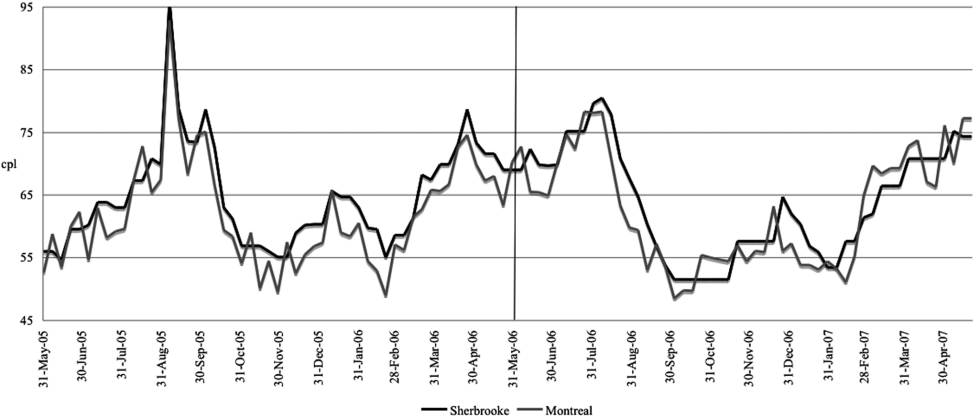
\includegraphics[width=0.92\textwidth]{figures/ch13/erutku2010_fig2.png}
\caption{Weekly retail prices net of taxes in Sherbrooke (black) and Montreal (gray), June 2005 to May 2007, in cents per liter. The
vertical line marks the announcement of the investigation at the end of May 2006. Source: \citet{ErutkuHildebrand2010}, Figure 2.}
\label{fig:13-eh-f2}
\end{figure}

The authors read the Montreal estimate as an overcharge of 1.75 cpl. Relative to the post-announcement Sherbrooke price, this is
$\frac{1.75}{64.0}=2.7$ percent of the retail price. Relative to the post-announcement margin over wholesale cost, it is
$\frac{1.75}{64.0-58.8}=34$ percent. About 135 million liters were sold in Sherbrooke between May 2005 and May 2006, so damages in the year
before the announcement exceed \$2 million ($0.0175\times135$ million $=\$2.4$ million, our arithmetic). The 2.7 percent overcharge is small
next to surveys of cartel overcharges (their Table~7, reproduced in \cref{tab:13-overcharge-surveys}), but the increase in the markup is
large. The authors compare it with Ohio school milk (p.~235). There \citet{PorterZona1999} estimate an average price effect of 6.5
percent, which they translate into a rise of roughly 30 percent in the markup (\cref{sec:13-pz99}). A cartel under investigation may also
keep prices high to reduce estimated damages \citep{Harrington2004}, so the estimate could understate the effect.

\casehead{Critiques}
The design rests on the choice of control. Quebec City matched Sherbrooke in levels before the announcement and moved with it after.
Either Quebec City prices were also affected by the investigation, or the Montreal estimate reflects Montreal-specific shocks. The data
cannot tell these apart. Parallel trends are checked only visually. There is one treated city and one control city in each regression,
so inference treats the weekly observations of a single pair as independent apart from an AR(1) correction. The general problems of
difference in differences with a single treated unit apply (\cref{app:econometrics}). The cartel's end date is uncertain, because
cooperation may have weakened when the wiretaps or raids began. Prices at the end of a cartel need not return at once to the competitive
level. \citet[p.~121]{ClarkHoude2013} report that their companion paper \citep{ClarkHoude2014} finds larger price cuts after the
collapse, which suggests a complementary reading. The cartel's main effect may have been on the shape of the cycle more than on the
average price.

\subsection{Learning to coordinate in Perth: Byrne and de Roos (2019)}\label{sec:13-perth}

The Quebec cartel coordinated by telephone. Coordinating a price increase took on average 65 calls among its members
and a price decrease 26 \citep[pp.~195--196]{AskerNocke2021}. Theory allows firms to reach the same outcome tacitly,
but it says little about how independent firms would arrive at a common understanding (p.~189).
\citet{ByrneDeRoos2019} document such a process in retail gasoline in Perth, Australia, from 2001 to 2015, as
summarized by \citet[pp.~189--191]{AskerNocke2021}. During this period, stations in Perth had to commit to their prices a
day ahead and post them on Fuelwatch, a government website. Its purpose was to help consumers find cheap gasoline.
The same transparency let stations monitor one another, which makes Fuelwatch a form of government-assisted
information sharing like the Danish publication of concrete prices (\cref{sec:13-concrete}).

Perth prices follow cycles of sudden jumps and gradual declines, like those of Toronto (\cref{sec:13-noel}). Before
2009, price jumps occurred on various days of the week. From 2009, BP, the largest chain, led jumps on Wednesdays.
Most of its remaining stations jumped on Thursdays. Caltex, the next-largest chain, gradually adopted the pattern,
and by mid-2010 it followed BP's Wednesday jump with a jump on Thursday. BP then reduced the share of its stations
that jumped on Wednesday and raised the share that jumped on Thursday. It thus scaled back its price leadership, and
with it the sales it lost by leading. In several periods BP stopped leading on Wednesday to test whether the market
would coordinate on Thursday without it (pp.~189--191, Figure~3). Byrne and de Roos identify two focal points
\citep[pp.~596--597 and 607--608]{ByrneDeRoos2019}. The first fixes the timing of the weekly price jump, which moved
to Thursday. The second fixes the size of the daily price cuts between jumps, which converged to 2 cents per liter
from March 2010. By 2013 adjustments were better synchronized and margins were higher.

The episode suggests a third kind of conduct behind similar price cycles. In Toronto the cycles were consistent with
competitive Edgeworth cycles. In Quebec an explicit cartel ran them by telephone. In Perth, the price data show a
detailed pattern of price leadership and price experiments under a transparency regime. The pattern is consistent
with coordination learned through prices. It does not show that prices were the only channel. Byrne and de Roos
state that they cannot rule out explicit communication between firms, such as phone calls
\citep[p.~617]{ByrneDeRoos2019}. Asker and Nocke distill the study as showing that market interaction itself \emph{may}
provide enough communication for coordination (p.~191). In terms of \cref{prop:13-transparency}, Fuelwatch raised the probability
that a deviation would be seen. The transition was slow. Asker and Nocke date it from 2009 to 2013 (p.~189).
Byrne and de Roos describe a gradual three-year transition from April 2009 to August 2012
\citep[p.~592]{ByrneDeRoos2019}, and in their conclusion they speak of three and a half years (p.~618). A simple
rule, such as a fixed day for jumps and a fixed size of cuts, makes deviations easy to detect. It also leaves the firms less able to respond to fluctuations in demand
\citep[p.~194]{AskerNocke2021}. \Cref{sec:12-anatomy} discusses the case as evidence on how agreements start.

\subsection{What the gasoline evidence shows}\label{sec:13-gas-synthesis}

\Cref{tab:13-gas-synthesis} summarizes the five studies. They share an industry, high-frequency prices and an observed wholesale cost.
They differ in what lets them speak about conduct. Borenstein and Shepard use a dynamic implication of the incentive constraint,
the response of margins to expected future demand and cost. Sign restrictions and a placebo separate collusion from inventories and
from measurement error. Noel uses the roles that theory assigns to small and large firms within a cycle. Clark and Houde use wiretaps,
which reveal the conduct directly, and then use structural models to measure what the observed mechanism achieved. Erutku and
Hildebrand use the end of the cartel as an event. Byrne and de Roos follow the emergence of price leadership over time.

\begin{table}[htbp]
\centering
\caption{Retail gasoline studies of conduct}\label{tab:13-gas-synthesis}
\footnotesize
\begin{tabularx}{\textwidth}{>{\raggedright\arraybackslash}p{2.0cm}>{\raggedright\arraybackslash}p{2.3cm}>{\raggedright\arraybackslash}X>{\raggedright\arraybackslash}X>{\raggedright\arraybackslash}X}
\toprule
Study & Market and data & Price pattern & Method & Conclusion about conduct\\
\midrule
\citet{BorensteinShepard1996} & 59 U.S. cities, monthly, 1986--1991 & Margins rise ahead of seasonal demand peaks and fall ahead of cost increases & 2SLS margin regression with forecast demand and cost, elasticity-corrected instrument, placebo on unexpected changes & Tacit dynamic collusion: margin elasticities of 0.37 to expected demand and $-0.37$ to expected cost (Table 2)\\
\addlinespace
\citet{Noel2007} & 22 Toronto stations, twelve-hourly, 131 days in 2001 & Asymmetric weekly cycle: one-step jumps of 5.6 cpl, then 12.8 half-days of small cuts & Markov-switching regression with sticky prices, leader and follower roles by firm type & Competitive Edgeworth cycles: small firms lead cuts, large firms lead relents (Tables II--V)\\
\addlinespace
\citet{ClarkHoude2013} & 128 stations in four Quebec cities, wiretaps 2005--2006, weekly prices 2002--2005 & Asymmetric cycle: increases near 4 cpl, cuts of 1--2 cpl, sticky prices & Coded court documents, delay regressions, logit and homogeneous demand, simulated incentive constraints & Explicit cartel using timed delays as transfers to low-cost firms: 4--6 percent volume gains (Table 7), shorter required punishments (Table 8)\\
\addlinespace
\citet{ErutkuHildebrand2010} & Sherbrooke versus Montreal and Quebec City, weekly, 2005--2007 & Price drop after the announcement of the investigation & Difference in differences with wholesale-price controls and AR(1) errors & Overcharge of 1.75 cpl against Montreal, none against Quebec City (Table 6)\\
\addlinespace
\citet{ByrneDeRoos2019} & Perth, daily station prices posted a day ahead on Fuelwatch, 2001--2015 & Cycles whose jumps moved to Thursdays after 2009 & Event history of price leadership and experimentation by BP & Coordination consistent with signaling through prices, explicit communication not ruled out: weekly jumps on Thursdays, daily cuts of 2 cpl and higher margins by 2013\\
\bottomrule
\end{tabularx}
\end{table}

Three lessons follow. First, price patterns alone do not identify conduct. Asymmetric cycles appear in competitive Toronto and in the
Quebec cartel, and parallel, synchronized increases arise in both. Perth adds cycles that the authors attribute to coordination through prices. Screens based on asymmetry, stickiness or low price variance
\citep{AbrantesMetzEtAl2006} can flag markets for scrutiny, but they cannot separate the two. Second, evidence becomes informative when
it tests a prediction specific to one theory. Examples are the expected-future effects of an incentive constraint, the role
assignments of the Maskin-Tirole equilibrium, or the transfers needed when firms are asymmetric. Third, direct evidence remains decisive
in prosecutions. The Quebec case rested on wiretaps and guilty pleas, and economic analysis then measured the mechanism and its
effects. \Cref{sec:13-enforcement} returns to these methods for measuring damages.
